\documentclass[conference,a4paper]{IEEEtran}

% ---------------------------------------------------------------
% Packages
% ---------------------------------------------------------------
\usepackage[T1]{fontenc}
\usepackage[utf8]{inputenc}
\usepackage{graphicx}
\usepackage{booktabs}
\usepackage{tabularx}
\usepackage{array}
\usepackage{makecell}
\usepackage{amsmath}
\usepackage{placeins}
\usepackage{xcolor}
\usepackage{microtype}
\usepackage[hidelinks]{hyperref}
\usepackage{url}

\newcolumntype{L}{>{\raggedright\arraybackslash}X}
\newcolumntype{P}[1]{>{\raggedright\arraybackslash}p{#1}}
\newcommand{\var}[1]{\texttt{#1}}
% Plain-language reading note placed under a table
\newcommand{\tabnote}[1]{\par\vspace{3pt}\begin{minipage}{\linewidth}\footnotesize\raggedright #1\end{minipage}}
\graphicspath{{figures/}{../figures/}}
\renewcommand{\arraystretch}{1.12}
\setlength{\emergencystretch}{3em}
% let LaTeX place several floats per page so no page is left half empty
\renewcommand{\topfraction}{0.9}
\renewcommand{\bottomfraction}{0.8}
\renewcommand{\textfraction}{0.07}
\renewcommand{\floatpagefraction}{0.8}
\renewcommand{\dbltopfraction}{0.9}
\renewcommand{\dblfloatpagefraction}{0.8}
\setcounter{topnumber}{3}
\setcounter{bottomnumber}{3}
\setcounter{totalnumber}{5}
\setcounter{dbltopnumber}{3}
\setlength{\dbltextfloatsep}{10pt plus 2pt minus 2pt}
\setlength{\dblfloatsep}{10pt plus 2pt minus 2pt}
\sloppy

\begin{document}

\title{ElimuSentry - Phase 1: Preparing the Data\\
\large How the data were checked, cleaned and planned for modelling, and why}

\author{\IEEEauthorblockN{Emile Lucky Muhigira}
\IEEEauthorblockA{Carnegie Mellon University Africa, Kigali, Rwanda\\
emuhigir@andrew.cmu.edu\\
04-652 Artificial Intelligence System Design, Assignment 2, Phase 1 (Preprocessing \& Feature Engineering Strategy)\\
Repository: \url{https://github.com/Emile-Lucky-Muhigira/AISD_Project}}}

\maketitle

\begin{abstract}
ElimuSentry is an early-warning system for school dropout. For a child aged 8--13 who is in school when a household survey visits, it estimates whether the child will be out of school at the next visit, about four years later, without having finished basic education. This report covers the step before any model is built: checking the data, finding and fixing problems, and deciding, with evidence, how every piece of information will be prepared. The data come from the Ghana Socioeconomic Panel Survey, which visited the same households in 2009/10, 2013/14 and 2017/18. Relevant modules from a download containing 317 Stata files were joined into one row per child. Children first seen in 2009/10 are used to build the model (1,307 children, 14.4\% dropped out); children first seen in 2013/14 form a later cohort for retrospective evaluation (1,395 children, 10.4\% dropped out). Each child is described by 33 pieces of information (``features''). The main findings: almost every child in the model-building table has at least one missing answer (only 4.1\% are complete), most measurements are lopsided rather than bell-shaped, and three features repeat information already held by others. The plan corrects recording errors with fixed rules, fills gaps with a method chosen for the reason each gap exists, tames extreme values instead of deleting children, removes the three redundant features (33 $\rightarrow$ 30), converts categories into numbers sensibly, and tests the model on a later time period with safeguards that stop test information leaking into training.
\end{abstract}

\begin{IEEEkeywords}
school dropout, early warning, data preprocessing, missing data, outliers, data leakage, Ghana panel survey
\end{IEEEkeywords}

% ===============================================================
\section{Introduction: Problem, Data and Repository}
% ===============================================================
\textbf{Problem.} School dropout in Sub-Saharan Africa usually happens gradually: absences pile up and learning falls behind before a child leaves \cite{balfanz2007}. The aim is to warn early, using information collected while the child is still in school (attendance, test results, household wealth, parents' education, school conditions), and to explain each warning in plain terms \cite{shap}. This supports Sustainable Development Goal 4 (targets 4.1 and 4.5).

\textbf{Data.} Ghana Socioeconomic Panel Survey, Waves 1--3 (2009/10, 2013/14, 2017/18), by ISSER (University of Ghana), Yale University and Northwestern University \cite{gsps}. The download contains 317 Stata files (one per questionnaire section per visit), linked by a household number and a person number.

\textbf{What is predicted, and what type of task this is.} \textbf{Dropout = 1} if the child is out of school at the next visit without having finished Junior Secondary School (JSS3); \textbf{0} if still in school. This is a \textbf{binary classification} task (two possible outcomes), and dropouts are the smaller group.

\textbf{Repository and reproducibility.} The GitHub repository follows the structure required by the assignment. Raw and processed data are kept out of GitHub by the \var{.gitignore} file (the raw download is 113\,MB, above GitHub's 100\,MB limit) and can be downloaded from the source link in the README. Two notebooks reproduce everything: \var{notebooks/01\_build\_dataset.ipynb} joins the survey files into the analysis tables, and \var{notebooks/02\_phase1\_audit.ipynb} produces every number, table and figure in this report (result tables are also saved in \var{phase1\_strategy/}). Software versions are fixed in \var{requirements.txt} (Python 3.11, pandas 3.0.6, scikit-learn 1.9.1, xgboost 3.2.0, pyreadstat 1.3.6).

\textbf{Reading this report.} The assignment requires several technical terms; each is explained in plain language in the Appendix at the end, just before the references. Sections II--IV follow the assignment's parts A, B and C.

% ===============================================================
\section{Dataset and Problem Audit (Part A)}
% ===============================================================
\begin{figure*}[!t]
\renewcommand{\thefigure}{0}
\centering
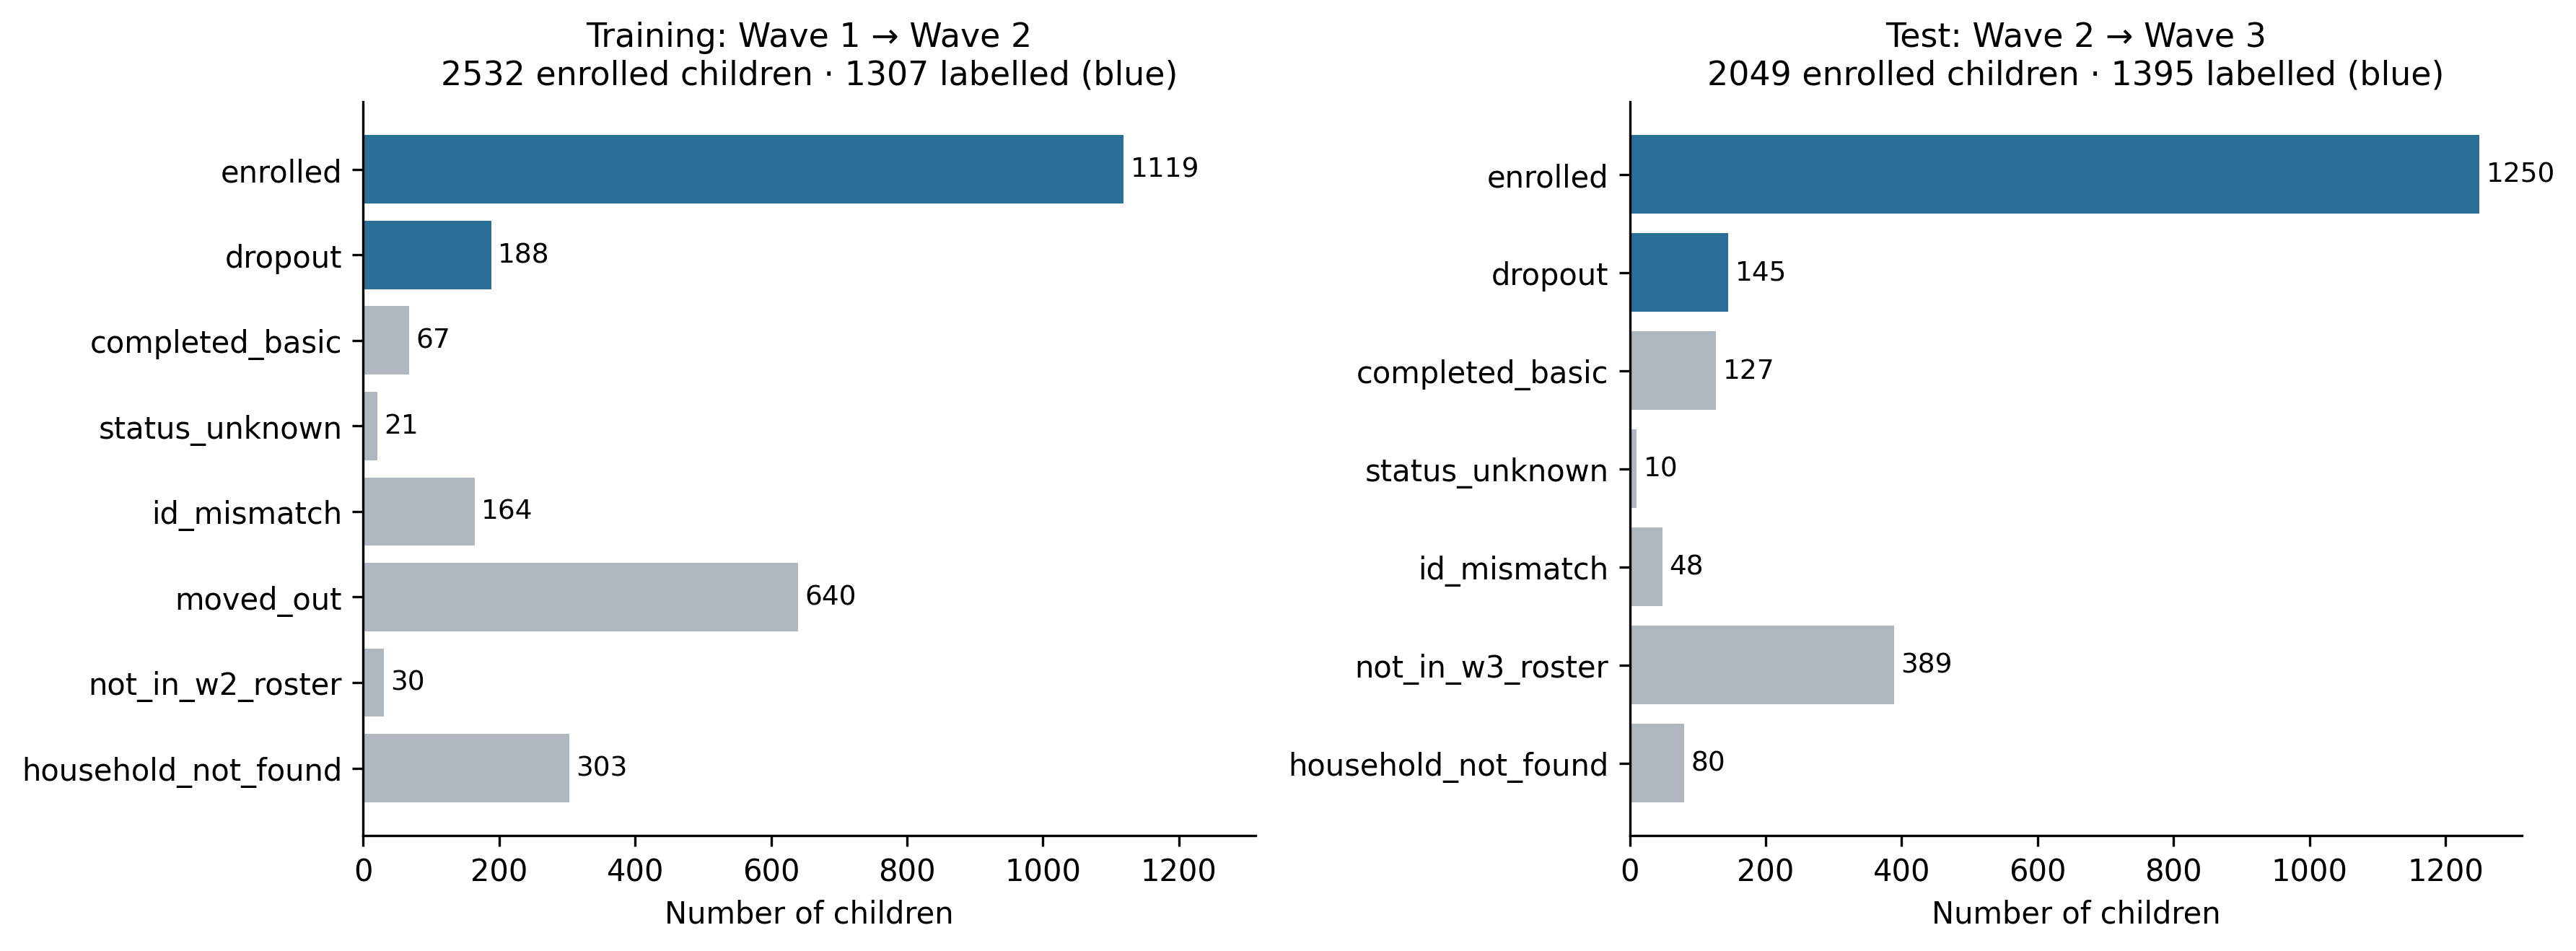
\includegraphics[width=\textwidth]{fig0_sample_flow.png}
\caption{What happened to every child who was in school at the first visit. Each bar is one possible outcome at the next visit; blue bars are the children whose outcome is known and who are used. Grey bars (labels as in the chart): household not found again (\var{household\_not\_found}); child no longer on the household list (\var{not\_in\_w2\_roster}, \var{not\_in\_w3\_roster}); child moved away (\var{moved\_out}); identity check failed, i.e.\ sex or age did not match (\var{id\_mismatch}); school status unknown (\var{status\_unknown}); finished basic education (\var{completed\_basic}). Of 2,532 children in school in 2009/10, 1,307 are used; of 2,049 in school in 2013/14, 1,395 are used. Far more children were lost in the first period because the 2017/18 survey, unlike the 2013/14 one, followed people who had moved into new households.}
\label{fig:flow}
\end{figure*}



\subsection*{A1. Size of the data}
There is no single ready-made table, so the ``starting size'' is that of the table built from the survey files: one row per child (Table~\ref{tab:shape}). For reference, the raw data are much larger: 317 Stata files, of which the 2009/10 person roster alone has 18,889 rows $\times$ 49 columns. Of all the people surveyed, 2,532 children aged 8--13 were in school in 2009/10 and 2,049 in 2013/14. Each child is followed from one visit to the next, and is accepted as the same person only if the sex matches and the age has gone up by 2--7 years. Children who finished basic education, could not be found again, failed this identity check, or had no school answer at the next visit are not used for modelling (Fig.~\ref{fig:flow}).

\begin{table}[!t]
\centering
\caption{Size of the two tables (A1)}
\label{tab:shape}
\footnotesize
\setlength{\tabcolsep}{4pt}
\begin{tabular}{lrrrr}
\toprule
Table & \makecell{Children\\(rows, $N$)} & \makecell{Features\\($P$)} & \makecell{House-\\holds} & \makecell{Dis-\\tricts} \\
\midrule
\makecell[l]{Model building\\(2009/10 $\rightarrow$ 2013/14)} & 1,307 & 33 & 1,014 & 136 \\
\makecell[l]{Testing\\(2013/14 $\rightarrow$ 2017/18)} & 1,395 & 33 & 1,091 & 137 \\
\bottomrule
\end{tabular}
\tabnote{Each table has 39 columns: 33 features + 5 identifier/weight columns + the target.}
\end{table}

\begin{table*}[!t]
\centering
\caption{All 39 columns, their meaning and type (A2)}
\label{tab:inventory}
\footnotesize
\begin{tabularx}{\textwidth}{P{3.3cm} L P{6.2cm}}
\toprule
Type (what it means) & Features in plain words & Code names \\
\midrule
\textbf{Continuous} (measured amounts) & Hours attended last week; hours missed last week; daily travel time to school (minutes); spending on the child's schooling (cedis per year); value of household goods (cedis); people per room & \var{attend\_hours}, \var{missed\_hours}, \var{travel\_minutes}, \var{school\_spend}, \var{durables\_value}, \var{persons\_per\_room} \\
\textbf{Discrete} (counts and scores) & Age (8--13); years older than normal for the grade ($-3$ to 7); math score (0--8); English reading score (0--7); days the teacher is absent per month; household size; number of 10 key assets owned; number of rooms & \var{age}, \var{over\_age}, \var{math\_score}, \var{english\_score}, \var{teacher\_absent\_days}, \var{hh\_size}, \var{asset\_count}, \var{rooms} \\
\textbf{Ordinal} (ordered categories) & School grade (preschool to JSS3); father's and mother's education (none to post-secondary); has textbooks (all / some / none) & \var{grade\_level}, \var{father\_edu}, \var{mother\_edu}, \var{has\_textbooks} \\
\textbf{Nominal} (labels, no order) & Region (10); school type (public/private, religious or not); relationship to household head; math and English test taken? (scored / blank sheet / not tested) & \var{regioncode}, \var{school\_type}, \var{relationship\_to\_head}, \var{math\_status}, \var{english\_status} \\
\textbf{Binary nominal} (yes / no labels) & Sex; urban or rural; recorded/inferred holiday or no-class week; in a school feeding programme; father alive; mother alive; father lives at home; mother lives at home; lost a parent; has electricity & \var{sex}, \var{urbrur}, \var{on\_vacation}, \var{feeding\_program}, \var{father\_alive}, \var{mother\_alive}, \var{father\_in\_hh}, \var{mother\_in\_hh}, \var{orphan}, \var{electricity} \\
\textbf{Date / free text} & None & n/a \\
\midrule
Identifiers (nominal codes; not used to predict) & Household number; person number; district; enumeration area (survey village) & \var{FPrimary}, \var{hhmid}, \var{district\_id}, \var{eacode} \\
Survey weight (continuous; not used to predict) & How many households each surveyed household represents & \var{hhweight3} \\
Target (binary) & Dropped out (1) or still in school (0) & \var{dropout} \\
\bottomrule
\end{tabularx}
\tabnote{Code names are those used in the notebooks. Full table: \var{A2\_variable\_inventory.csv}.}
\end{table*}

\textbf{Problems found while building the table} (details in \var{notebooks/01\_build\_dataset.ipynb}): some files used an old Windows text format; most numbers were stored as text; codes changed between visits (e.g.\ sex was recorded as 1/2 in 2009/10 but 1/5 in 2013/14) and were made consistent; 2 duplicate people were removed; district numbers repeat across regions (112 different codes stand for 136 real districts in the model-building table and 137 in the testing table), so region and district were combined into one district code; test answers were stored as letters or codes rather than right/wrong, so they were marked with an answer key recovered from the 2017/18 survey (it matches the most common answer on every question); and the question on a parent's education was skipped when the parent lives in the same household, so that parent's own education record was used instead (apparent missing information on father's education fell from about 54\% to 7.7\%). The derived orphan indicator is 1 when either parent is known deceased, 0 only when both are known alive, and missing otherwise (27 model-building records and one testing record). A parent living elsewhere can still be alive.

\subsection*{A2. What kind of information each column holds}
\begin{table*}[!t]
\centering
\caption{Missing answers before fixed value corrections (A3a)}
\label{tab:missing}
\footnotesize
\setlength{\tabcolsep}{4pt}
\begin{tabular}{lrr|rr@{\hskip 16pt}lrr|rr}
\toprule
 & \multicolumn{2}{c|}{Model building} & \multicolumn{2}{c}{Testing} & & \multicolumn{2}{c|}{Model building} & \multicolumn{2}{c}{Testing} \\
Feature & Missing & \% & Missing & \% & Feature & Missing & \% & Missing & \% \\
\midrule
Hours missed last week & 1016 & 77.7 & 12 & 0.9 & Travel time & 28 & 2.1 & 12 & 0.9 \\
Days teacher absent & 743 & 56.8 & 441 & 31.6 & Mother alive & 20 & 1.5 & 1 & 0.1 \\
English score & 716 & 54.8 & 557 & 39.9 & School spending & 20 & 1.5 & 0 & 0.0 \\
Math score & 437 & 33.4 & 340 & 24.4 & Mother lives at home & 20 & 1.5 & 1 & 0.1 \\
Hours attended last week & 282 & 21.6 & 12 & 0.9 & Has electricity & 17 & 1.3 & 1 & 0.1 \\
Father's education & 101 & 7.7 & 75 & 5.4 & Father lives at home & 14 & 1.1 & 1 & 0.1 \\
School type & 84 & 6.4 & 0 & 0.0 & Father alive & 14 & 1.1 & 1 & 0.1 \\
School grade & 81 & 6.2 & 7 & 0.5 & Feeding programme & 11 & 0.8 & 1 & 0.1 \\
Years over-age for grade & 81 & 6.2 & 7 & 0.5 & People per room & 5 & 0.4 & 4 & 0.3 \\
Mother's education & 50 & 3.8 & 27 & 1.9 & Number of rooms & 5 & 0.4 & 2 & 0.1 \\
Has textbooks & 34 & 2.6 & 1 & 0.1 & Value of goods & 5 & 0.4 & 9 & 0.6 \\
Lost a parent (derived) & 27 & 2.1 & 1 & 0.1 & Key assets owned & 5 & 0.4 & 0 & 0.0 \\
\bottomrule
\end{tabular}
\tabnote{Features not listed have no gaps at this baseline stage. All 39 columns, including identifiers, weight and target, are reported in \var{A3\_baseline\_missingness.csv}; the corrected-feature profile is in \var{A3\_missingness.csv}.}
\end{table*}

\begin{figure*}[!t]
\renewcommand{\thefigure}{1.1}
\centering
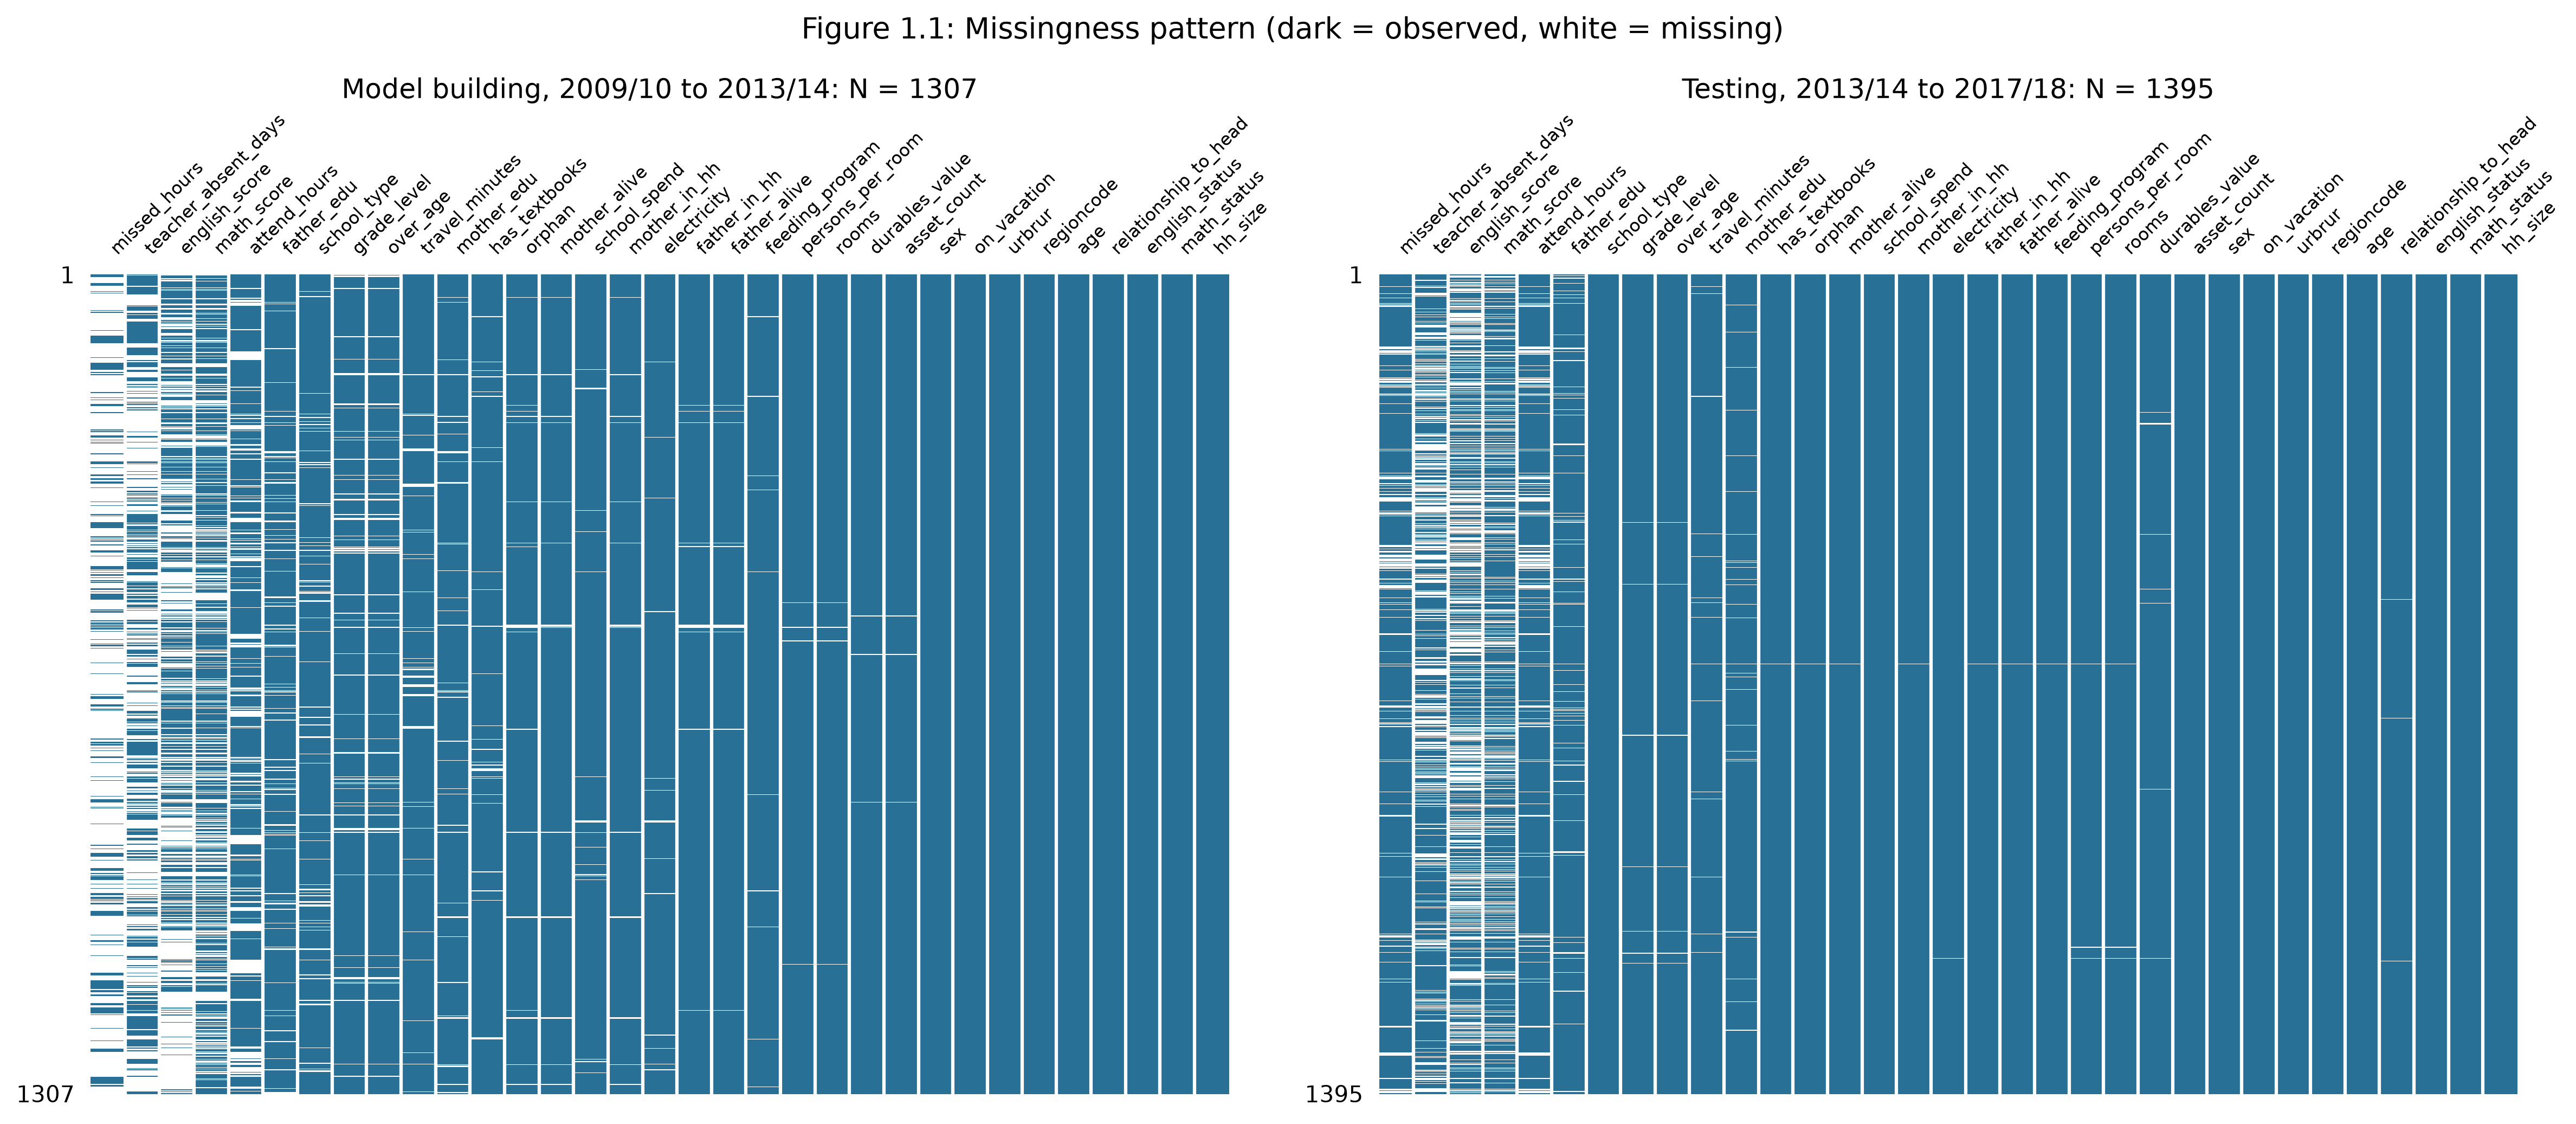
\includegraphics[width=0.92\textwidth]{fig1_1_missingness_heatmap.png}
\caption{Where answers are missing after fixed value corrections, before imputation. Left: model-building table; right: testing table. \emph{How to read it:} each thin row is one child and each column is one feature; a white mark means that answer is missing. Columns are sorted from most to least missing, so in the model-building table the large white blocks on the left are hours missed (78\% missing), days teacher absent (57\%), English score (55\%), math score (33\%) and hours attended (22\%). Most other columns are almost fully filled.}
\label{fig:missing}
\end{figure*}

Each column is classified by what its values \emph{mean}, not by how the computer stores them. For example, region is stored as a number from 1 to 10, but region 8 is not ``more'' than region 4; it is a label. Yes/no items are nominal labels with only two options; they are listed in their own row because they are handled more simply (0/1). No feature is a date or free text (Table~\ref{tab:inventory}). Counts: 6 continuous, 8 discrete, 4 ordinal, 15 nominal (5 with several options + 10 yes/no), 0 date/text = 33 features.

\subsection*{A3. Baseline and corrected missingness}
The baseline is the linked and harmonised child-level matrix, after recognising survey special codes but \textbf{before fixed value corrections}, filling, capping or scaling. Linkage, category harmonisation and feature construction are necessary to define these 33 features; this is not an untouched raw survey module. The original Stata files are unaltered. Separate \var{*\_pre\_correction.csv} snapshots preserve this stage. Table~\ref{tab:missing} gives the baseline counts per feature; identifiers, weight and target have no gaps.

\textbf{Before fixed value corrections:} 3,816 of 43,131 feature cells (8.85\%) are missing in training; 1,513 of 46,035 (3.29\%) in testing. There are 54 complete training rows (4.1\%) and 1,253 with at least one gap; testing has 512 complete rows (36.7\%) and 883 with gaps. Using all 39 columns as the denominator gives 3,816/50,973 (7.49\%) and 1,513/54,405 (2.78\%), respectively.

\textbf{After fixed value corrections, before filling:} training has 3,847 missing feature cells (8.92\%), 53 complete rows and 1,254 incomplete rows; testing has 1,827 (3.97\%), 467 complete and 928 incomplete rows. Across all 39 columns these percentages are 7.55\% and 3.36\%. Nine training features and 11 testing features have no gaps. These are the inputs for the strategy in B1 and Fig.~\ref{fig:missing}, not the pre-correction baseline. The summary for both stages and denominators is saved in \var{A3\_missingness\_summary.csv}. The survey modes and the inferred Wave 2 no-class-week rule both contribute to the difference between periods.

\subsection*{A4. The outcome to predict}
The task is binary classification. Table~\ref{tab:target} gives the class balance and the class imbalance ratio; Fig.~\ref{fig:target} shows it.

\begin{table}[!t]
\centering
\caption{How many children dropped out (A4)}
\label{tab:target}
\footnotesize
\setlength{\tabcolsep}{2.4pt}
\begin{tabular}{lrrrr}
\toprule
Table & \makecell{Stayed\\(0)} & \makecell{Dropped\\out (1)} & \makecell{Dropout\\rate} & \makecell{Imbalance\\ratio} \\
\midrule
\makecell[l]{Model building\\(2009/10 $\rightarrow$ 2013/14)} & 1,119 & 188 & 14.4\% & 5.95 : 1 \\
\makecell[l]{Testing\\(2013/14 $\rightarrow$ 2017/18)} & 1,250 & 145 & 10.4\% & 8.62 : 1 \\
\bottomrule
\end{tabular}
\tabnote{Imbalance ratio = children who stayed : children who dropped out. In training, each dropout is given this ratio as extra weight ($\approx$6$\times$; see text).}
\end{table}

\begin{figure}[!t]
\renewcommand{\thefigure}{1.2}
\centering
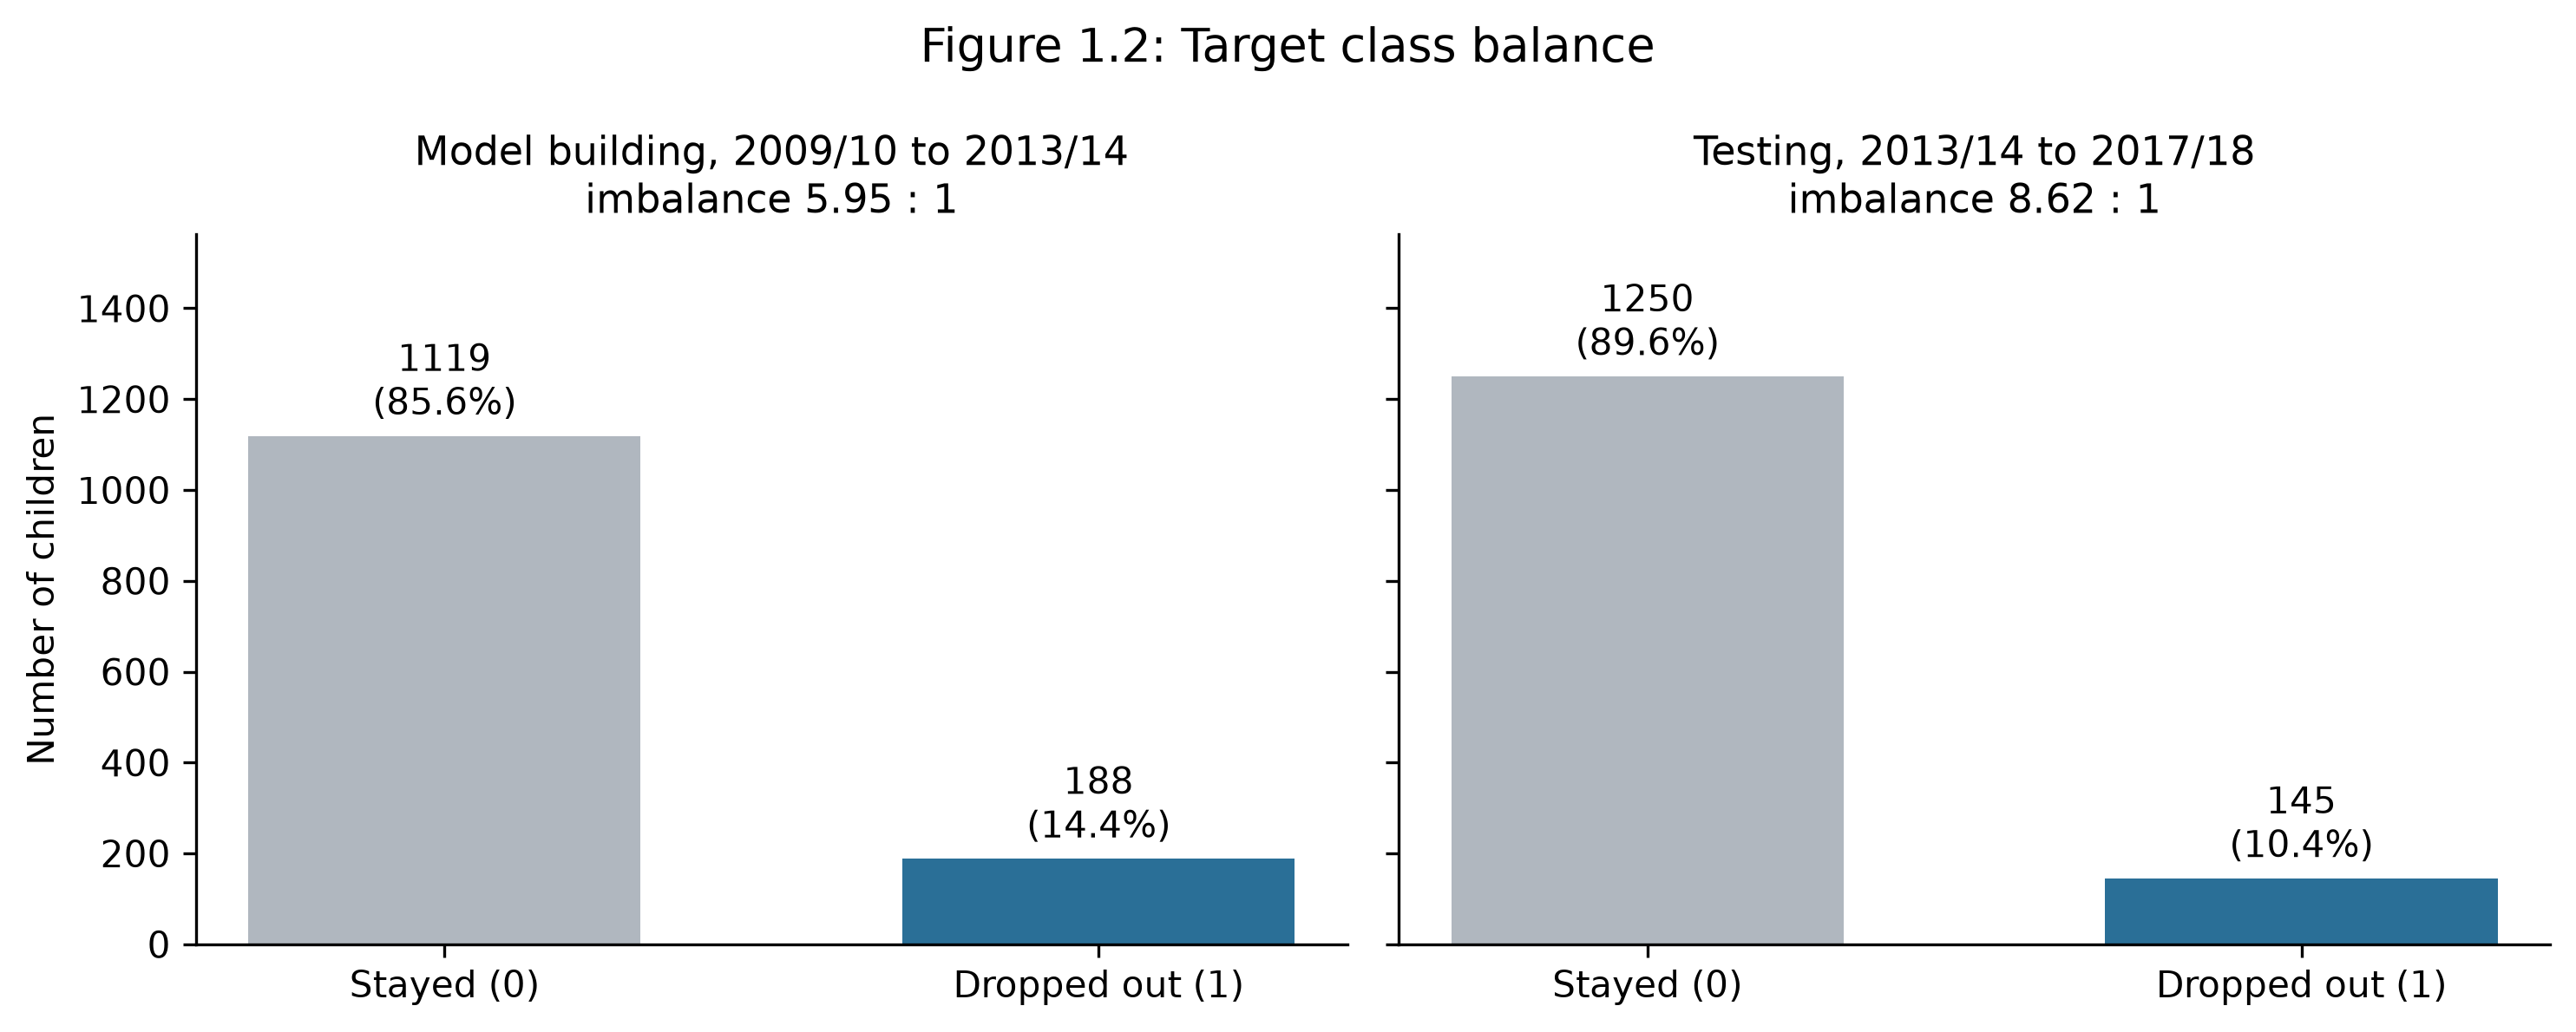
\includegraphics[width=\columnwidth]{fig1_2_target_distribution.png}
\caption{Children still in school vs dropped out. Left: model-building table (1,119 stayed, 188 dropped out = 14.4\%). Right: testing table (1,250 stayed, 145 dropped out = 10.4\%). The short bars show that dropouts are the small group.}
\label{fig:target}
\end{figure}

\textbf{How the imbalance is handled.} Dropouts are the minority (about 1 in 7), so a ``model'' that simply says nobody drops out would already be right 85.6\% of the time while being useless. Accuracy is therefore not used to judge the model; instead we measure how well it ranks the real dropouts near the top of its list (PR-AUC) and how many dropouts are caught when the top 20\% riskiest children are flagged \cite{saito2015}. During training, each dropout is given about 6 times the weight of a child who stays in school (\emph{class weighting}: \var{scale\_pos\_weight} in XGBoost \cite{xgboost}, \var{class\_weight="balanced"} in logistic regression), recalculated within each fold. We do \emph{not} create copies or artificial dropouts (over-sampling, SMOTE): weighting gives the same balancing effect without adding made-up children, and each made-up child would be built by mixing real children, often siblings or neighbours, which could carry their information across the checks in C2. Because the extra weight pushes risk scores upwards, the risk percentages will be re-adjusted (calibrated) before use \cite{zadrozny2002}, using only 2009/10 predictions on the checking folds and never test outcomes. No adjustment is learned from later-period outcomes; the lower observed dropout rate (10.4\% instead of 14.4\%) is reported as a limitation (Section~\ref{sec:limits}).

% ===============================================================
\section{Cleaning and Imputation Strategy (Part B)}
% ===============================================================
\begin{table*}[!t]
\centering
\caption{Why each feature has gaps and how they will be filled (B1)}
\label{tab:b1}
\footnotesize
\setlength{\tabcolsep}{4pt}
\begin{tabularx}{\textwidth}{P{3.0cm} r r r P{6.6cm} L}
\toprule
Feature & \makecell{Missing\\\%} & \makecell{Gap linked\\to dropout? ($p$)} & \makecell{Lopsided?\\(skew)} & Why it is missing (type and evidence) & How the gap is filled \\
\midrule
Hours missed last week & 77.8 & 0.665 & 1.93 & \textbf{Uncertain; possibly MNAR}: a blank could mean zero missed hours, but the questionnaire does not establish this. Similar positive-report rates (15.7\% vs 14.4\%) and no detected dropout association do not identify the missing values. Compare zero filling with median filling inside validation & Set to 0 when attendance was recorded; otherwise middle value (median). No extra flag under the retained assumption; assess this choice in sensitivity analysis \\
Days teacher absent & 56.8 & $7.7\times10^{-4}$ & 2.95 & \textbf{MAR} (by questionnaire design): asked only if the child has one main teacher, which depends on the grade we can see (89--100\% missing in JSS). Observed dropout differs descriptively (17.2\% vs 10.6\%); the flag is justified by questionnaire design & Median (= 0) + ``was missing'' flag \\
English score & 54.8 & 0.205 & $-0.32$ & \textbf{MAR}: children under 9 were not tested by design; gaps also more common in northern, rural and poorer areas. Possible \textbf{MNAR} for blank answer sheets; a blank alone does not establish reading ability & Average (mean) + keep ``test taken?'' (scored / blank / not tested) \\
Math score & 33.4 & 0.233 & $-0.14$ & \textbf{MAR} on age and region; Possible \textbf{MNAR} for blank sheets (descriptive dropout 36\% vs 14\%, 22 children); mechanism unverified & Average (mean) + keep ``test taken?'' \\
Hours attended last week & 21.8 & 0.181 & $-0.96$ & Plausible \textbf{MAR} on recorded holiday/region in Wave 1; the Wave 2 zero/zero-hours flag is only an inferred no-class-week proxy & Median + holiday flag + ``was missing'' flag \\
Father's education & 7.7 & 0.181 & 0.34 & \textbf{MAR}: ``don't know'' about a father who lives elsewhere (more common in urban, wealthier homes); the gap itself describes the child's family situation & Most common answer (mode) + ``was missing'' flag \\
School type & 6.4 & 0.208 & n/a & \textbf{MAR} on region & Separate ``missing'' option \\
School grade & 6.2 & 0.233 & 0.29 & \textbf{MAR} on region & Mixed-distance KNN; k selected using inner district-grouped training folds \\
Years over-age for grade & 6.2 & 0.233 & 0.30 & \textbf{MAR}: missing exactly when grade is missing & Recalculated from the estimated grade \\
Travel time & 4.2 & 0.972 & 3.15 & \textbf{MAR} on region and mother at home & Median \\
Mother's education & 3.8 & 0.118 & 0.71 & \textbf{MAR}: ``don't know'' about a mother who lives elsewhere; the gap itself describes the child's family situation & Mode + ``was missing'' flag \\
School spending & 1.5 & 0.192 & 10.78 & \textbf{MAR} on age, urban, wealth & Median \\
Has electricity & 1.3 & 0.026 & n/a & Compatible with \textbf{MCAR}, not proof: no link to other answers; the dropout link rests on 17 children and may be chance & Mode \\
Has textbooks; mother alive; mother at home; feeding programme & $\le$2.6 & $>$0.2 & n/a & Compatible with \textbf{MCAR}, not proof (no link, or one weak chance-level link) & Mode \\
Lost a parent (derived) & 2.1 & 0.262 & 2.59 & Parent status unknown and neither parent known deceased; preserve this uncertainty & Removed as a derived feature in B4b \\
Father alive; father at home & 1.1 & 1.00 & n/a & \textbf{MAR} on urban and mother at home & Mode \\
Key assets; value of goods; rooms; people per room & 0.4 & 0.541--1.000 & $\ge$0.62 & Compatible with \textbf{MCAR}, not proof (household file not matched; one weak link for rooms) & Median \\
\bottomrule
\end{tabularx}
\tabnote{Raw $p$ values are exploratory; BH-adjusted missingness-screen $q$ values are in the companion CSV. Skew measures asymmetry; for numerical gaps the plan uses the median when $|\mathrm{skew}|\ge0.5$, the mean otherwise. Mechanisms remain working assumptions. Evidence: \var{B1\_missingness\_evidence.csv}, \var{B1\_missingness\_tests.csv}, \var{B1\_mechanism\_and\_imputation\_plan.csv}.}
\end{table*}

\subsection*{Fixing recording errors first}
\label{sec:corrections}
Special codes such as ```99 = on holiday'' are recognised as survey responses, not genuine measurements. Fixed plausibility and travel-box rules then correct suspected entry errors. The Wave 2 zero/zero-hours rule is a separate modelling assumption, not a confirmed recording error or holiday. These rules do not estimate parameters from either table (Table~\ref{tab:corrections}); their assumptions still require sensitivity checks. After the travel-time fix, the two tables agree closely (average 31.8 vs 32.4 minutes), which supports the rule.

\begin{table}[!t]
\centering
\caption{Rules used to fix recording errors}
\label{tab:corrections}
\footnotesize
\setlength{\tabcolsep}{3pt}
\begin{tabularx}{\columnwidth}{L r r}
\toprule
Rule & 2009/10 & 2013/14 \\
\midrule
Code 99 meant ``on holiday'' in the hours questions $\rightarrow$ marked missing, and a survey-coded holiday flag added & 183 & n/a \\
Inferred no-class week: 0 attended \emph{and} 0 missed $\rightarrow$ proxy flag, hours missing. Holiday interpretation is unverified & n/a & 221 \\
Travel time typed in the wrong box (e.g.\ ``30'' in the hours box with minutes blank) $\rightarrow$ read as minutes & 69 & 13 \\
Travel over 300 minutes a day (5-hour round trip, not compatible with daily school) $\rightarrow$ missing & 53 & 6 \\
More than 50 class hours attended in one week $\rightarrow$ missing & 5 & 0 \\
More than 50 class hours missed in one week $\rightarrow$ missing & 1 & 0 \\
Teacher absent more than 22 days in a month (more than the school days in a month) $\rightarrow$ missing & 2 & 4 \\
Household with 0 rooms $\rightarrow$ missing & 0 & 2 \\
Child aged 8--13 recorded as the spouse of the household head $\rightarrow$ missing & 2 & 3 \\
\bottomrule
\end{tabularx}
\tabnote{Counts are out of all 2,532 (2009/10) and 2,049 (2013/14) children in school at the first visit, before the samples were reduced to 1,307 and 1,395, so they are larger than the counts in later tables.}
\end{table}

\subsection*{B1. Why information is missing, and how each gap will be filled}
\begin{table*}[!t]
\centering
\caption{Screening for extreme values in the model-building table (B2)}
\label{tab:b2}
\footnotesize
\setlength{\tabcolsep}{5pt}
\begin{tabular}{lrrrrrr}
\toprule
Feature & \makecell{Lopsided?\\(skew)} & \makecell{Share of\\zeros \%} & \makecell{Normal range by\\IQR rule (raw)} & \makecell{Flagged by\\IQR rule} & \makecell{Flagged by\\Z-score rule} & \makecell{Flagged by IQR\\after log transform} \\
\midrule
Hours attended last week & $-0.96$ & 0.3 & 10.0 to 50.0 & 132 & 0 & 145 \\
Hours missed last week & 1.93 & 37.2 & up to 17.5 & 38 & 5 & 0 \\
Travel time (min) & 3.15 & 0.2 & up to 85.0 & 77 & 13 & 5 \\
School spending (cedis) & 10.78 & 0.3 & up to 363.7 & 115 & 18 & 5 \\
Value of household goods (cedis) & 10.05 & 0.1 & up to 2,310.9 & 146 & 13 & 14 \\
People per room & 1.10 & 0.0 & up to 7.8 & 35 & 20 & 0 \\
Days teacher absent & 2.95 & 74.8 & up to 2.5 & 67 & 15 & 35 \\
Household size & 1.31 & 0.0 & up to 11.5 & 33 & 23 & 6 \\
Number of rooms & 4.82 & 0.0 & up to 8.5 & 74 & 27 & 5 \\
Key assets owned & 0.62 & 10.0 & up to 8.5 & 7 & 1 & 0 \\
Years over-age for grade & 0.30 & 15.7 & $-2.0$ to 6.0 & 2 & 2 & 0 \\
Age; math score; English score & below 0.33 & n/a & fixed scales & 0 & 0 & n/a \\
\bottomrule
\end{tabular}
\tabnote{\emph{How to read it:} the last three columns give how many children each rule would call ``extreme''. The raw IQR rule flags many believable values; a Gaussian tail interpretation of the Z-score rule is inappropriate for these distributions; the IQR rule applied after the log transform (last column) flags only a few, and is the rule used; the two exceptions are handled separately in Table~\ref{tab:b3}. Counts include unusually low values; only the high end is capped (B3). For hours attended, the 145 flagged values are \emph{very low} attendance (under 15 hours a week), which is kept as a warning sign; for days teacher absent, 75\% of values are 0, so the rule does not work. Full table: \var{B2\_outlier\_screening.csv}.}
\end{table*}

\textbf{Evidence and uncertainty.} Missingness is screened against age, sex, urban/rural, northern region, assets, mother present and dropout. Numeric covariates use Mann--Whitney; categorical ones use Pearson chi-square only when all expected cells are at least 5, otherwise Fisher exact or fixed-margin Monte Carlo \cite{scipyfisher}. All estimable missingness screens form one BH-adjusted family, with a BY sensitivity \cite{scipyfdr}; raw $p$, adjusted $q$, expected counts and method are saved in \var{B1\_missingness\_tests.csv}. The B1 table shows raw exploratory $p$ values, not claims of confirmed associations. Mechanisms are working assumptions from survey design and domain reasoning: plausible MAR when observed circumstances may explain gaps; possible MNAR when the hidden value may matter; MCAR-compatible where no clear pattern is detected. Neither an association nor its absence proves a mechanism \cite{rubin1976,littlerubin}. Low missingness does not guarantee negligible bias. The four missing indicators are fixed from questionnaire/family context, not selected using validation outcomes.

\textbf{Rules for filling gaps}, applied the same way everywhere:
\begin{itemize}
\item Numbers that are roughly balanced ($|$skew$|<0.5$) $\rightarrow$ fill with the \textbf{average} (mean).
\item Numbers with a long tail ($|$skew$|\ge0.5$) $\rightarrow$ fill with the \textbf{middle value} (median), which a few extreme values cannot pull.
\item Yes/no items and ordered categories $\rightarrow$ fill with the \textbf{most common answer} (mode).
\item Labels whose gaps carry meaning $\rightarrow$ add a separate ``missing'' option.
\item When the gap itself tells us something (it follows from the questionnaire design, it describes the family situation, or family context justifies retaining the gap), a yes/no \textbf{``was missing'' flag} is added so the model can use that fact, unless there are fewer than 20 gaps (too few for a flag to be learned) or an explicit alternative is assessed (zero-filling hours missed versus median filling).
\item School grade $\rightarrow$ estimated by \textbf{mixed-distance KNN}. Age and key assets use absolute differences divided by ranges learned from training donors only, capped at 1. Sex, urban/rural and region use 0 for the same category and 1 for a different category: changing a region's numeric code cannot change the distance. Each variable has equal weight; average only the comparisons observed in both children. Include every donor tied at the kth distance, average their grades, round and bound to the valid 0--9 scale. If no comparison is available, use the training median grade. Preserve every observed grade and recalculate over-age for imputed grades.
\end{itemize}
All filling values are learned from the model-building part of each fold only (Section C2), never from the data used to check the model.

\textbf{How k is justified, without leakage.} Candidate neighbour counts are 3, 5, 9, 15 and 25: a small predeclared grid covering local estimates and more stable smoothing. Inside every pipeline fit, use three district-grouped inner folds of the observed training grades and select the k with the lowest pooled mean absolute grade error (MAE); an exact tie favours the larger k. All ranges and donors are learned again inside each inner fit. Neither dropout, over-age nor any temporal test data enter this selection. Full-training inner scores for k=3,5,9,15,25 are respectively 1.254, 1.216, 1.172, 1.156 and 1.179 grades, selecting \textbf{k=15}; this number is not forced into other fits.

\textbf{Independent grade-recovery check.} Five outer district-grouped folds hide each observed validation grade and its derived over-age value. The corrected method selects k again within the outer training districts, then recovers the hidden grades. There are 1,226 held-out observed grades in total, with no shared districts at either validation level. This is a validation experiment on the model-building table, not a use of the temporal test set. Outer fits select k=15 or 25.

\begin{table}[!t]
\centering
\caption{Training-only nested grade-imputation validation}
\label{tab:knn}
\footnotesize
\setlength{\tabcolsep}{3pt}
\begin{tabularx}{\columnwidth}{L r r r}
\toprule
Method & \makecell{MAE\\(grades)} & \makecell{Exact\\grade \%} & \makecell{Within one\\grade \%} \\
\midrule
Training median & 1.444 & 22.3 & 58.6 \\
Legacy numeric-code KNN, k=5 & 1.110 & 27.7 & 71.5 \\
Mixed-distance KNN, inner-selected k & 1.128 & 28.2 & 70.0 \\
\bottomrule
\end{tabularx}
\tabnote{MAE is pooled across all 1,226 hidden observed grades. Smaller is better. The corrected distance reduces MAE by 21.9\% versus median filling, but is 0.018 grades worse than the legacy method; no accuracy advantage over the legacy method is claimed.}
\end{table}

The numerical-code method is retained only as a comparison: it imposes an ordering on nominal regions. The mixed distance has a defensible categorical interpretation regardless of that small error difference. This experiment cannot reveal the true error on the 81 genuinely missing training grades, whose missingness may differ from the observed cases. Tables are reproducible in the audit notebook, section B1.3 (\var{B1\_knn\_summary.csv}, \var{B1\_knn\_validation.csv}, \var{B1\_knn\_inner\_folds.csv}, \var{B1\_knn\_k\_selection.csv}). Behavioural checks verify invariance to category relabelling and donor order, preservation of observed grades, valid output grades, handling of missing predictors, and that transform learns nothing from query rows.

 The few gaps that appear only in the testing table (e.g.\ relationship to head, 3 children) are filled with the same rules, using values learned from model-building data.

\textbf{Why we do not simply delete children with gaps.} Only 4.1\% of children have no gap at all, so deleting incomplete rows would leave 53 children. It would also remove younger and northern children far more than others, exactly where the gaps concentrate.

\textbf{Children whose outcome is unknown.} Children who could not be found again are older and much less often live with their parents (father at home 52\% vs 67\%, mother 65\% vs 83\%, $p<10^{-11}$); grandchildren, foster children and other relatives were lost 54--59\% of the time, against 33\% for the head's own children. These observed differences show selective follow-up and possible selection bias. They do not identify the unobserved outcomes, establish MNAR rather than MAR, or determine whether the measured dropout rate is too high or too low. Unknown outcomes are not imputed as observed labels; this is reported as a limitation (Section~\ref{sec:limits}).

\subsection*{B2. Spotting extreme values (outliers)}
\begin{table*}[!t]
\centering
\caption{How extreme values are treated (B3)}
\label{tab:b3}
\footnotesize
\setlength{\tabcolsep}{4pt}
\begin{tabularx}{\textwidth}{P{4.0cm} P{3.6cm} r r r L}
\toprule
Feature & Treatment & \makecell{Upper\\limit} & \makecell{Values capped\\(building)} & \makecell{Values capped\\(testing)} & Reason \\
\midrule
Travel time (min) & Log, then cap & 294.0 & 2 & 0 & Long tail; the raw rule would cap 77 genuine long walks \\
School spending (cedis) & Replaced by a rank (C1) & (3,120.2) & n/a & n/a & Very long tail; the rank has fixed limits, so no cap is needed \\
Value of household goods (cedis) & Replaced by a rank (C1) & (17,123.4) & n/a & n/a & Very long tail; without inflation adjustment 74 test values would exceed the cap \\
Number of rooms & Log, then cap & 18.8 & 5 & 1 & Compound houses with up to 52 rooms \\
Household size & Log, then cap & 15.2 & 6 & 4 & Households with up to 20 people \\
Hours missed; people per room (removed in B4b) & Log only & n/a & 0 & 0 & Nothing extreme after the log \\
Hours attended last week & Not capped & n/a & n/a & n/a & Very low attendance is genuine and may signal risk; capping would hide it \\
Days teacher absent & Not capped & n/a & n/a & n/a & 75\% zeros, so the IQR rule breaks down; already limited to 0--22 \\
Age; years over-age; scores; key assets & Not capped & n/a & n/a & n/a & Fixed scales; every value is valid \\
\bottomrule
\end{tabularx}
\tabnote{Full table: \var{B3\_outlier\_treatment\_plan.csv}.}
\end{table*}

\begin{figure*}[!t]
\renewcommand{\thefigure}{2.1}
\centering
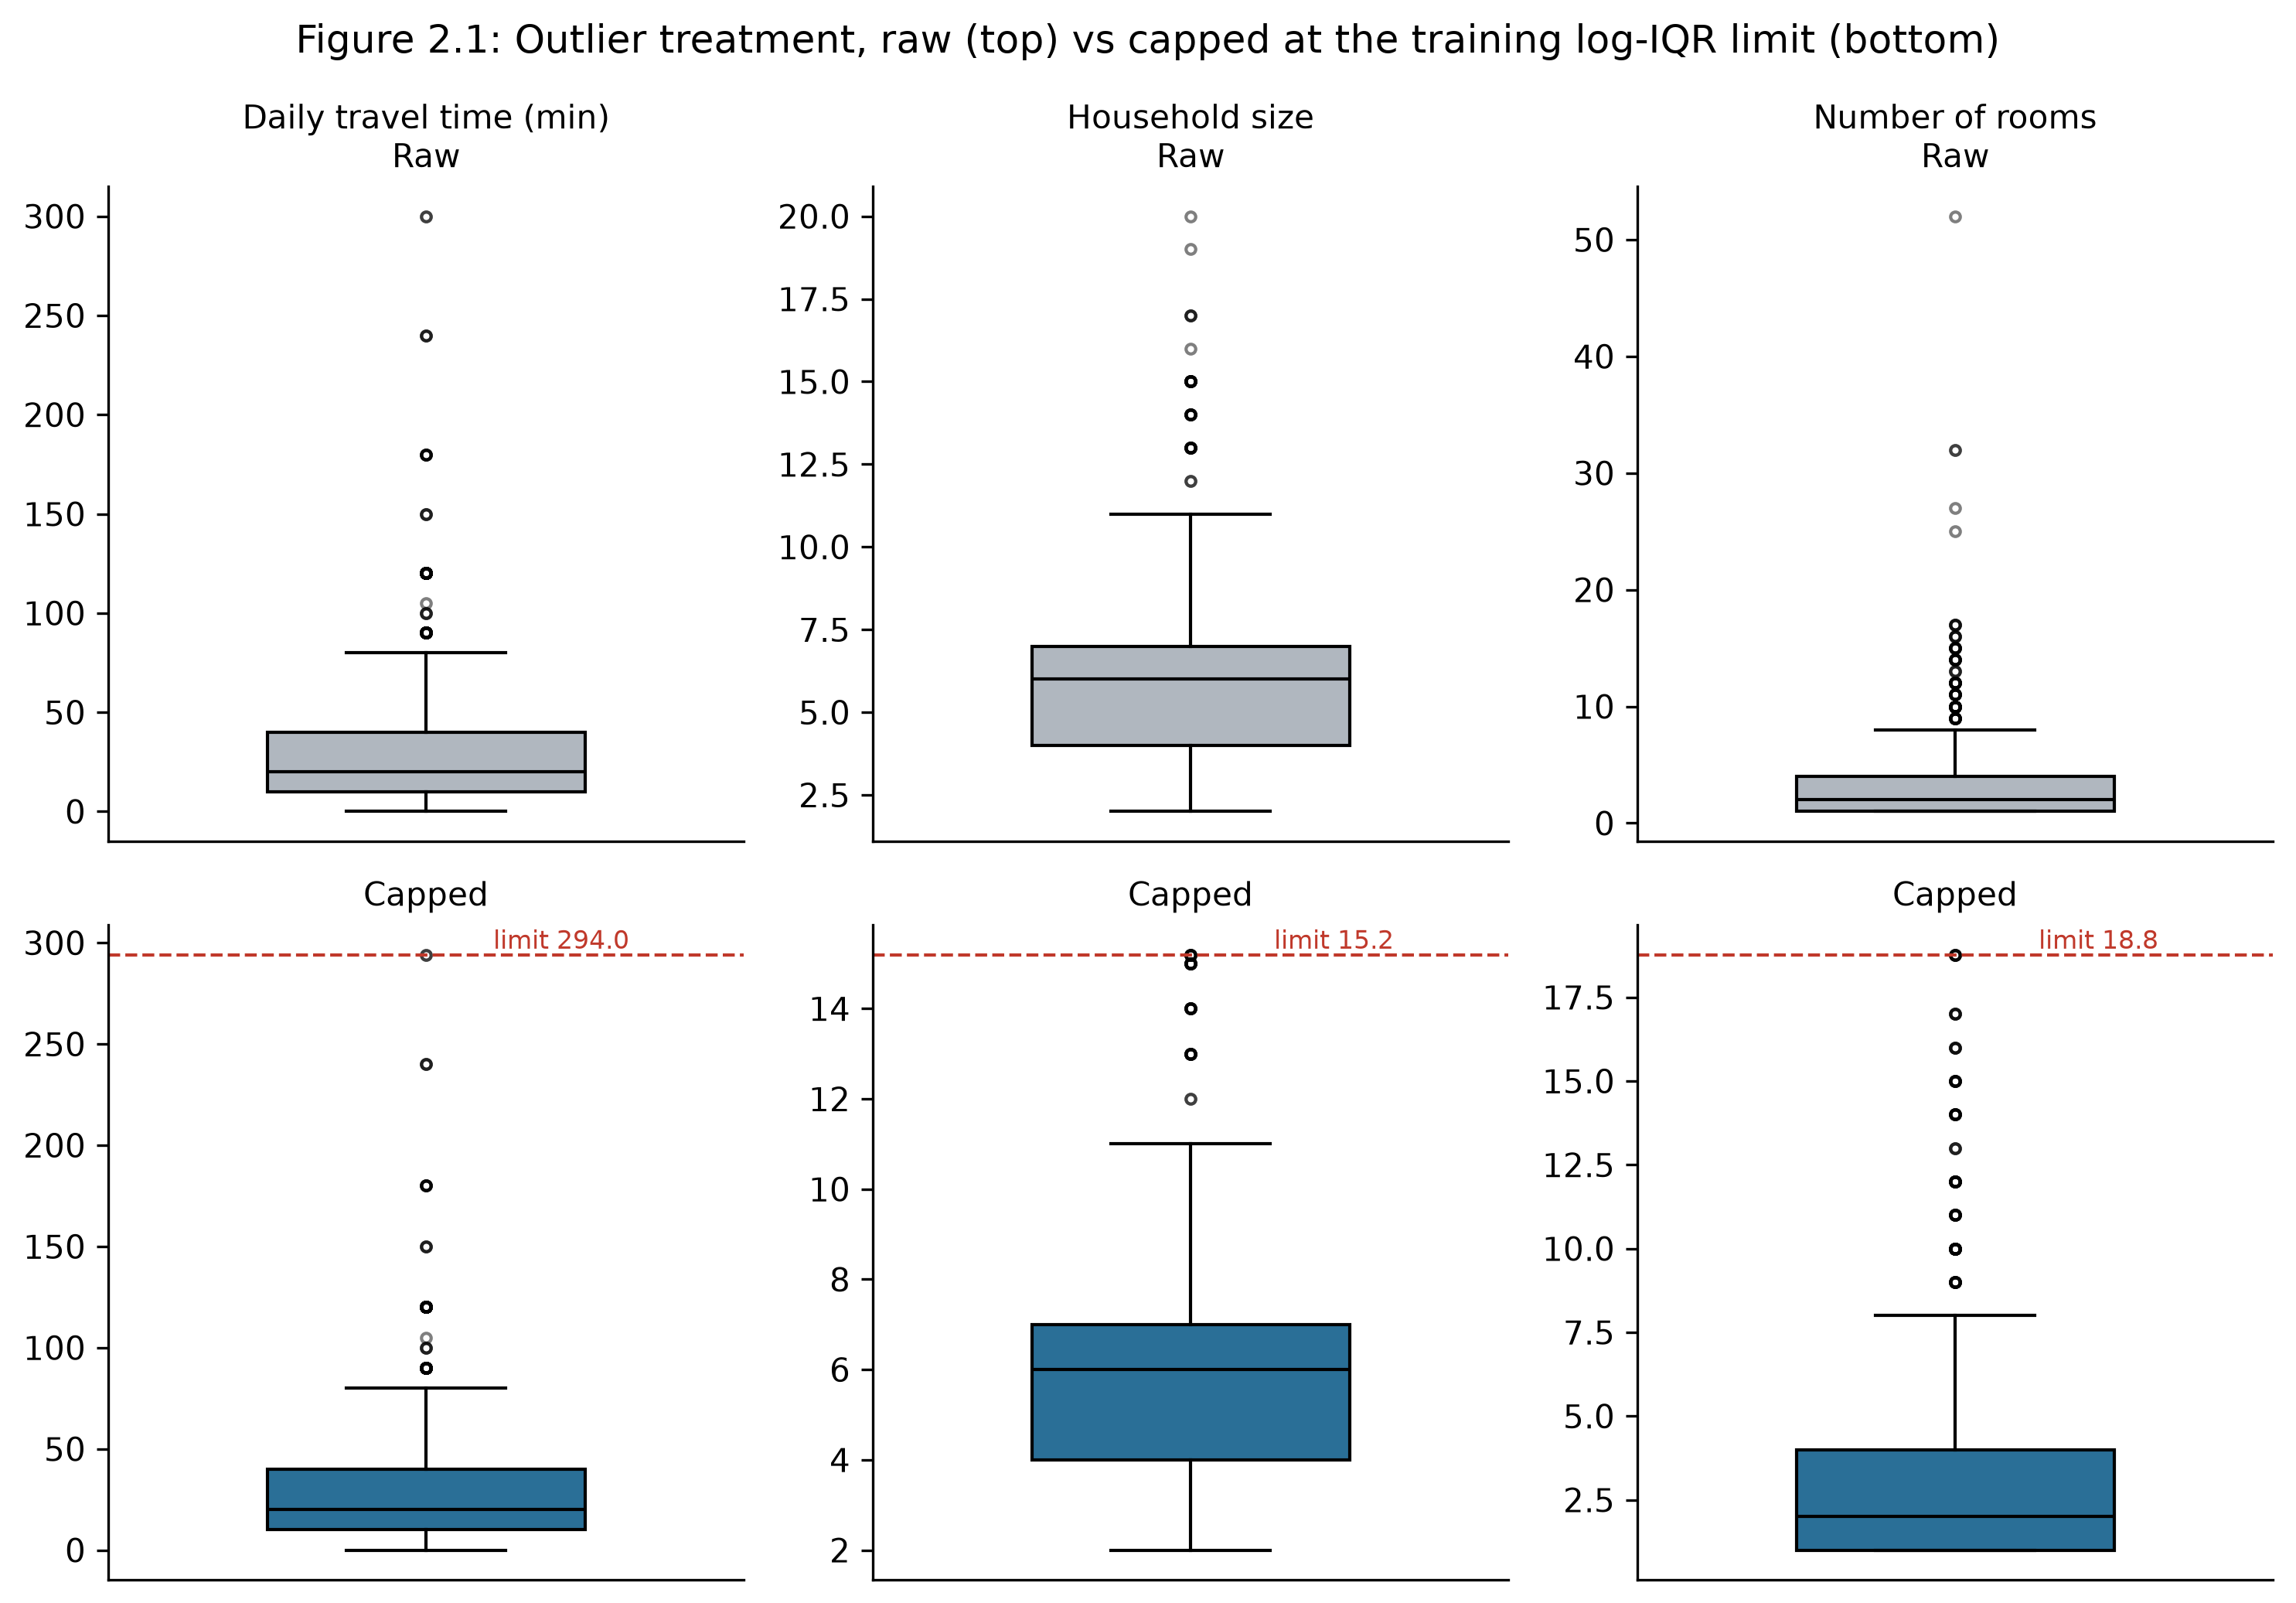
\includegraphics[width=0.92\textwidth]{fig2_1_outlier_boxplots.png}
\caption{Extreme values before and after capping for travel time, household size and rooms. Top: corrected input values. Bottom: values above the red dashed training-derived log-IQR limit are capped, with no row deleted. The two money features are ranked instead of capped and are not shown in this figure. Remaining dots follow the box plot's own reference rule and need not exceed the pipeline cap.}
\label{fig:outliers}
\end{figure*}

\textbf{Which rule.} The \textbf{Z-score rule} flags a value when $|Z| = |(x-\mu)/\sigma| > 3$, i.e.\ more than 3 standard deviations from the average. Z-scores are computable for any nonconstant numerical feature; the usual Gaussian tail interpretation assumes a bell shape. Every numeric feature failed the D'Agostino--Pearson test for a bell shape ($p<0.001$), so it is shown in Table~\ref{tab:b2} for comparison only. The \textbf{IQR rule} \cite{tukey} is used instead: a value is flagged if it lies more than 1.5 times the width of the middle half of the data beyond the edges of that middle half ($[Q_1-1.5\,\text{IQR},\,Q_3+1.5\,\text{IQR}]$). For example, the middle half of children travel between 10 and 40 minutes (a range of 30 minutes), so the rule flags anything above $40+1.5\times30=85$ minutes. Applied to the raw values, this rule flags many genuine high values in long-tailed features (77 children travelling more than 85 minutes, 146 household-goods values). After a log transform, which compresses the long tail, it flags only a handful, so the limits are computed on the log scale (Table~\ref{tab:b2}).

\subsection*{B3. Treating extreme values: capping, not deleting}
\begin{table*}[!t]
\centering
\caption{Exploratory feature--dropout associations, with multiplicity adjustment (B4a)}
\label{tab:b4a}
\footnotesize
\setlength{\tabcolsep}{4pt}
\renewcommand{\arraystretch}{1.0}
\begin{tabularx}{\textwidth}{P{3.1cm} P{1.6cm} c c r r r L}
\toprule
Feature & Type & Test & Effect & Raw $p$ & BH $q$ & MI & $q<0.05$ \\
\midrule
Region & Nominal & $\chi^2$ & $V=+0.295$ & $2.6\times10^{-20}$ & $8.6\times10^{-19}$ & 0.0367 & yes \\
Value of goods & Continuous & MW & $r=+0.066$ & 0.149 & 0.246 & 0.0213 & no \\
Rooms & Discrete & MW & $r=+0.165$ & $2.0\times10^{-4}$ & 0.001 & 0.0177 & yes \\
School spending & Continuous & MW & $r=-0.200$ & $1.4\times10^{-5}$ & $1.1\times10^{-4}$ & 0.0133 & yes \\
English score & Discrete & MW & $r=-0.245$ & $4.3\times10^{-4}$ & 0.002 & 0.0125 & yes \\
Household size & Discrete & MW & $r=+0.145$ & 0.001 & 0.004 & 0.0113 & yes \\
People per room & Continuous & MW & $r=-0.095$ & 0.036 & 0.080 & 0.0105 & no \\
Father's education & Ordinal & MW & $r=-0.203$ & $3.6\times10^{-6}$ & $6.0\times10^{-5}$ & 0.0102 & yes \\
Mother's education & Ordinal & MW & $r=-0.190$ & $9.0\times10^{-6}$ & $9.9\times10^{-5}$ & 0.0090 & yes \\
Teacher absence & Discrete & MW & $r=+0.041$ & 0.496 & 0.577 & 0.0078 & no \\
Years over-age & Discrete & MW & $r=+0.146$ & 0.001 & 0.004 & 0.0075 & yes \\
School type & Nominal & $\chi^2$ & $V=+0.108$ & 0.002 & 0.006 & 0.0062 & yes \\
Electricity & Binary & $\chi^2$ & $V=+0.105$ & $1.6\times10^{-4}$ & 0.001 & 0.0056 & yes \\
Travel time & Continuous & MW & $r=+0.039$ & 0.401 & 0.491 & 0.0053 & no \\
Father in household & Binary & $\chi^2$ & $V=+0.095$ & $6.1\times10^{-4}$ & 0.003 & 0.0048 & yes \\
Math score & Discrete & MW & $r=-0.038$ & 0.507 & 0.577 & 0.0047 & no \\
Urban/rural & Binary & $\chi^2$ & $V=+0.091$ & 0.001 & 0.004 & 0.0043 & yes \\
Key assets & Discrete & MW & $r=-0.043$ & 0.346 & 0.456 & 0.0043 & no \\
Hours missed & Continuous & MW & $r=+0.302$ & 0.001 & 0.004 & 0.0033 & yes \\
Age & Discrete & MW & $r=+0.041$ & 0.365 & 0.463 & 0.0031 & no \\
Math test status & Nominal & FMC & $V=+0.084$ & 0.018 & 0.042 & 0.0027 & yes \\
School grade & Ordinal & MW & $r=-0.061$ & 0.184 & 0.280 & 0.0019 & no \\
Father alive & Binary & $\chi^2$ & $V=+0.052$ & 0.063 & 0.122 & 0.0015 & no \\
Relationship to head & Nominal & FMC & $V=+0.050$ & 0.573 & 0.591 & 0.0015 & no \\
Feeding programme & Binary & $\chi^2$ & $V=+0.056$ & 0.044 & 0.090 & 0.0015 & no \\
English test status & Nominal & $\chi^2$ & $V=+0.047$ & 0.239 & 0.328 & 0.0010 & no \\
Holiday/no-class proxy & Binary & $\chi^2$ & $V=+0.040$ & 0.149 & 0.246 & 0.0009 & no \\
Textbooks & Ordinal & MW & $r=+0.052$ & 0.201 & 0.288 & 0.0008 & no \\
Orphan status & Binary & $\chi^2$ & $V=+0.037$ & 0.187 & 0.280 & 0.0007 & no \\
Sex & Binary & $\chi^2$ & $V=+0.017$ & 0.530 & 0.583 & 0.0002 & no \\
Mother in household & Binary & $\chi^2$ & $V=+0.016$ & 0.568 & 0.591 & 0.0001 & no \\
Mother alive & Binary & $\chi^2$ & $V=+0.011$ & 0.694 & 0.694 & 0.0001 & no \\
Hours attended & Continuous & MW & $r=-0.077$ & 0.136 & 0.246 & 0.0000 & no \\
\bottomrule
\end{tabularx}
\tabnote{MW = Mann--Whitney; FET = Fisher exact (2 by 2); FMC = fixed-margin Fisher Monte Carlo (99,999 samples, seed 42); $\chi^2$ = Pearson chi-square. Any expected cell below 5 routes to FET/FMC. $r$ is rank-biserial effect; $V$ uses uncorrected Pearson chi-square. BH adjusts all 33 tests as one family; a conservative Benjamini--Yekutieli (BY) sensitivity is saved alongside it. These row-level tests are exploratory, not survey-weighted or cluster-robust population inference. Full diagnostics: \var{B4a\_feature\_target\_tests.csv}.}
\end{table*}

Values above the limit are \textbf{capped}: pulled back down to the limit. The limit is found by applying the IQR rule to the log-transformed values and converting the result back to normal units; for travel time this gives 294 minutes (almost 5 hours), so only 2 children are capped instead of 77. (For the two money features the limits are shown for reference only; they are replaced by ranks in C1.) Only the high end is capped, because low values are genuine (no spending under free schooling, zero travel for boarders). \textbf{No child is deleted.} Deleting a whole child because one number is extreme would throw away its other answers, which still carry useful signal about dropout, and shrink the already small group of 188 dropouts, which lowers statistical power and makes the model more likely to overfit; and very large, very rich or very remote households are not random, so deleting them would make the data less like the real population. The limits are set using model-building data only and applied unchanged to the data used for checking (Table~\ref{tab:b3}).

Only 13 values are capped in the model-building table (5 in the testing table). The dots still visible in the lower panels of Fig.~\ref{fig:outliers} are within the limits; they appear only because the box plot draws its own reference lines on the raw scale.

\subsection*{B4a. Testing each feature against dropout}
\begin{table*}[!t]
\centering
\caption{Features removed because they repeat others (B4b)}
\label{tab:b4b}
\footnotesize
\begin{tabularx}{\textwidth}{P{3.0cm} P{4.2cm} r r L}
\toprule
Removed & Why it was flagged & \makecell{VIF\\before} & MI & Reason for removing this one \\
\midrule
People per room & Correlation $-0.855$ with number of rooms & 1.77 & 0.0105 & Calculated from household size and rooms; retain its two source measurements \\
Lost a parent & Correlation $-0.850$ with father alive & 20.21 & 0.0007 & Derived from parent-alive items; retain source items and preserve unknowns in the audit \\
School grade & VIF above 10: fully determined by age and years over-age & 19.86 & 0.0019 & Exactly equal to age $-$ years over-age $-$ 5, retain age and the domain-relevant over-age signal by a fixed rule \\
\midrule
\multicolumn{5}{P{0.97\textwidth}}{Highest VIF before removal: lost a parent 20.2, school grade 19.9, age 17.0, father alive 14.4, years over-age 14.1. \quad After removal: highest VIF = 1.89 (key assets), so none exceeds the declared VIF threshold.} \\
\bottomrule
\end{tabularx}
\tabnote{\emph{How to read it:} ``VIF before'' shows how much of the feature could already be predicted from all the others (above 10 = it adds almost nothing new); MI is how much it tells us about dropout (from Table~\ref{tab:b4a}). The removal list is fixed by feature construction and domain meaning; MI values are descriptive, not the selection rule. Full tables: \var{B4b\_multicollinearity\_drops.csv}, \var{B4b\_vif.csv}.}
\end{table*}

Each feature is tested using its measurement type. \textbf{Numbers and ordered categories}: Mann--Whitney compares rank distributions, with rank-biserial $r$ as effect size; it is not automatically a test of medians unless distribution shapes support that interpretation. \textbf{Nominal and binary features}: check expected cell counts first. Use Pearson chi-square when adequate, otherwise Fisher exact for 2 by 2 tables or a fixed-margin Monte Carlo Fisher test for larger sparse tables \cite{scipyfisher}. Cramer's $V$ is computed from uncorrected Pearson chi-square as a descriptive effect size regardless of the p-value method. \textbf{All features}: MI describes predictive association, and all 33 p-values are adjusted as one BH family; BY is a more conservative dependence sensitivity \cite{scipyfdr}. Pearson correlation can be computed without Gaussian predictors; the rank method is chosen for robustness to skew and extremes, not because normality is required to calculate a correlation. Tests are exploratory, not causal, survey-weighted or cluster-robust inference.

\textbf{Reading the table.} It reports raw $p$ and adjusted $q$ separately. A BH $q<0.05$ is an exploratory flag after multiplicity adjustment, not proof of a relationship. The BY sensitivity and small-cell diagnostics are in the CSV. No feature is selected or removed by these p-values; structural removals remain fixed before validation.

\begin{figure}[!t]
\renewcommand{\thefigure}{3.3}
\centering
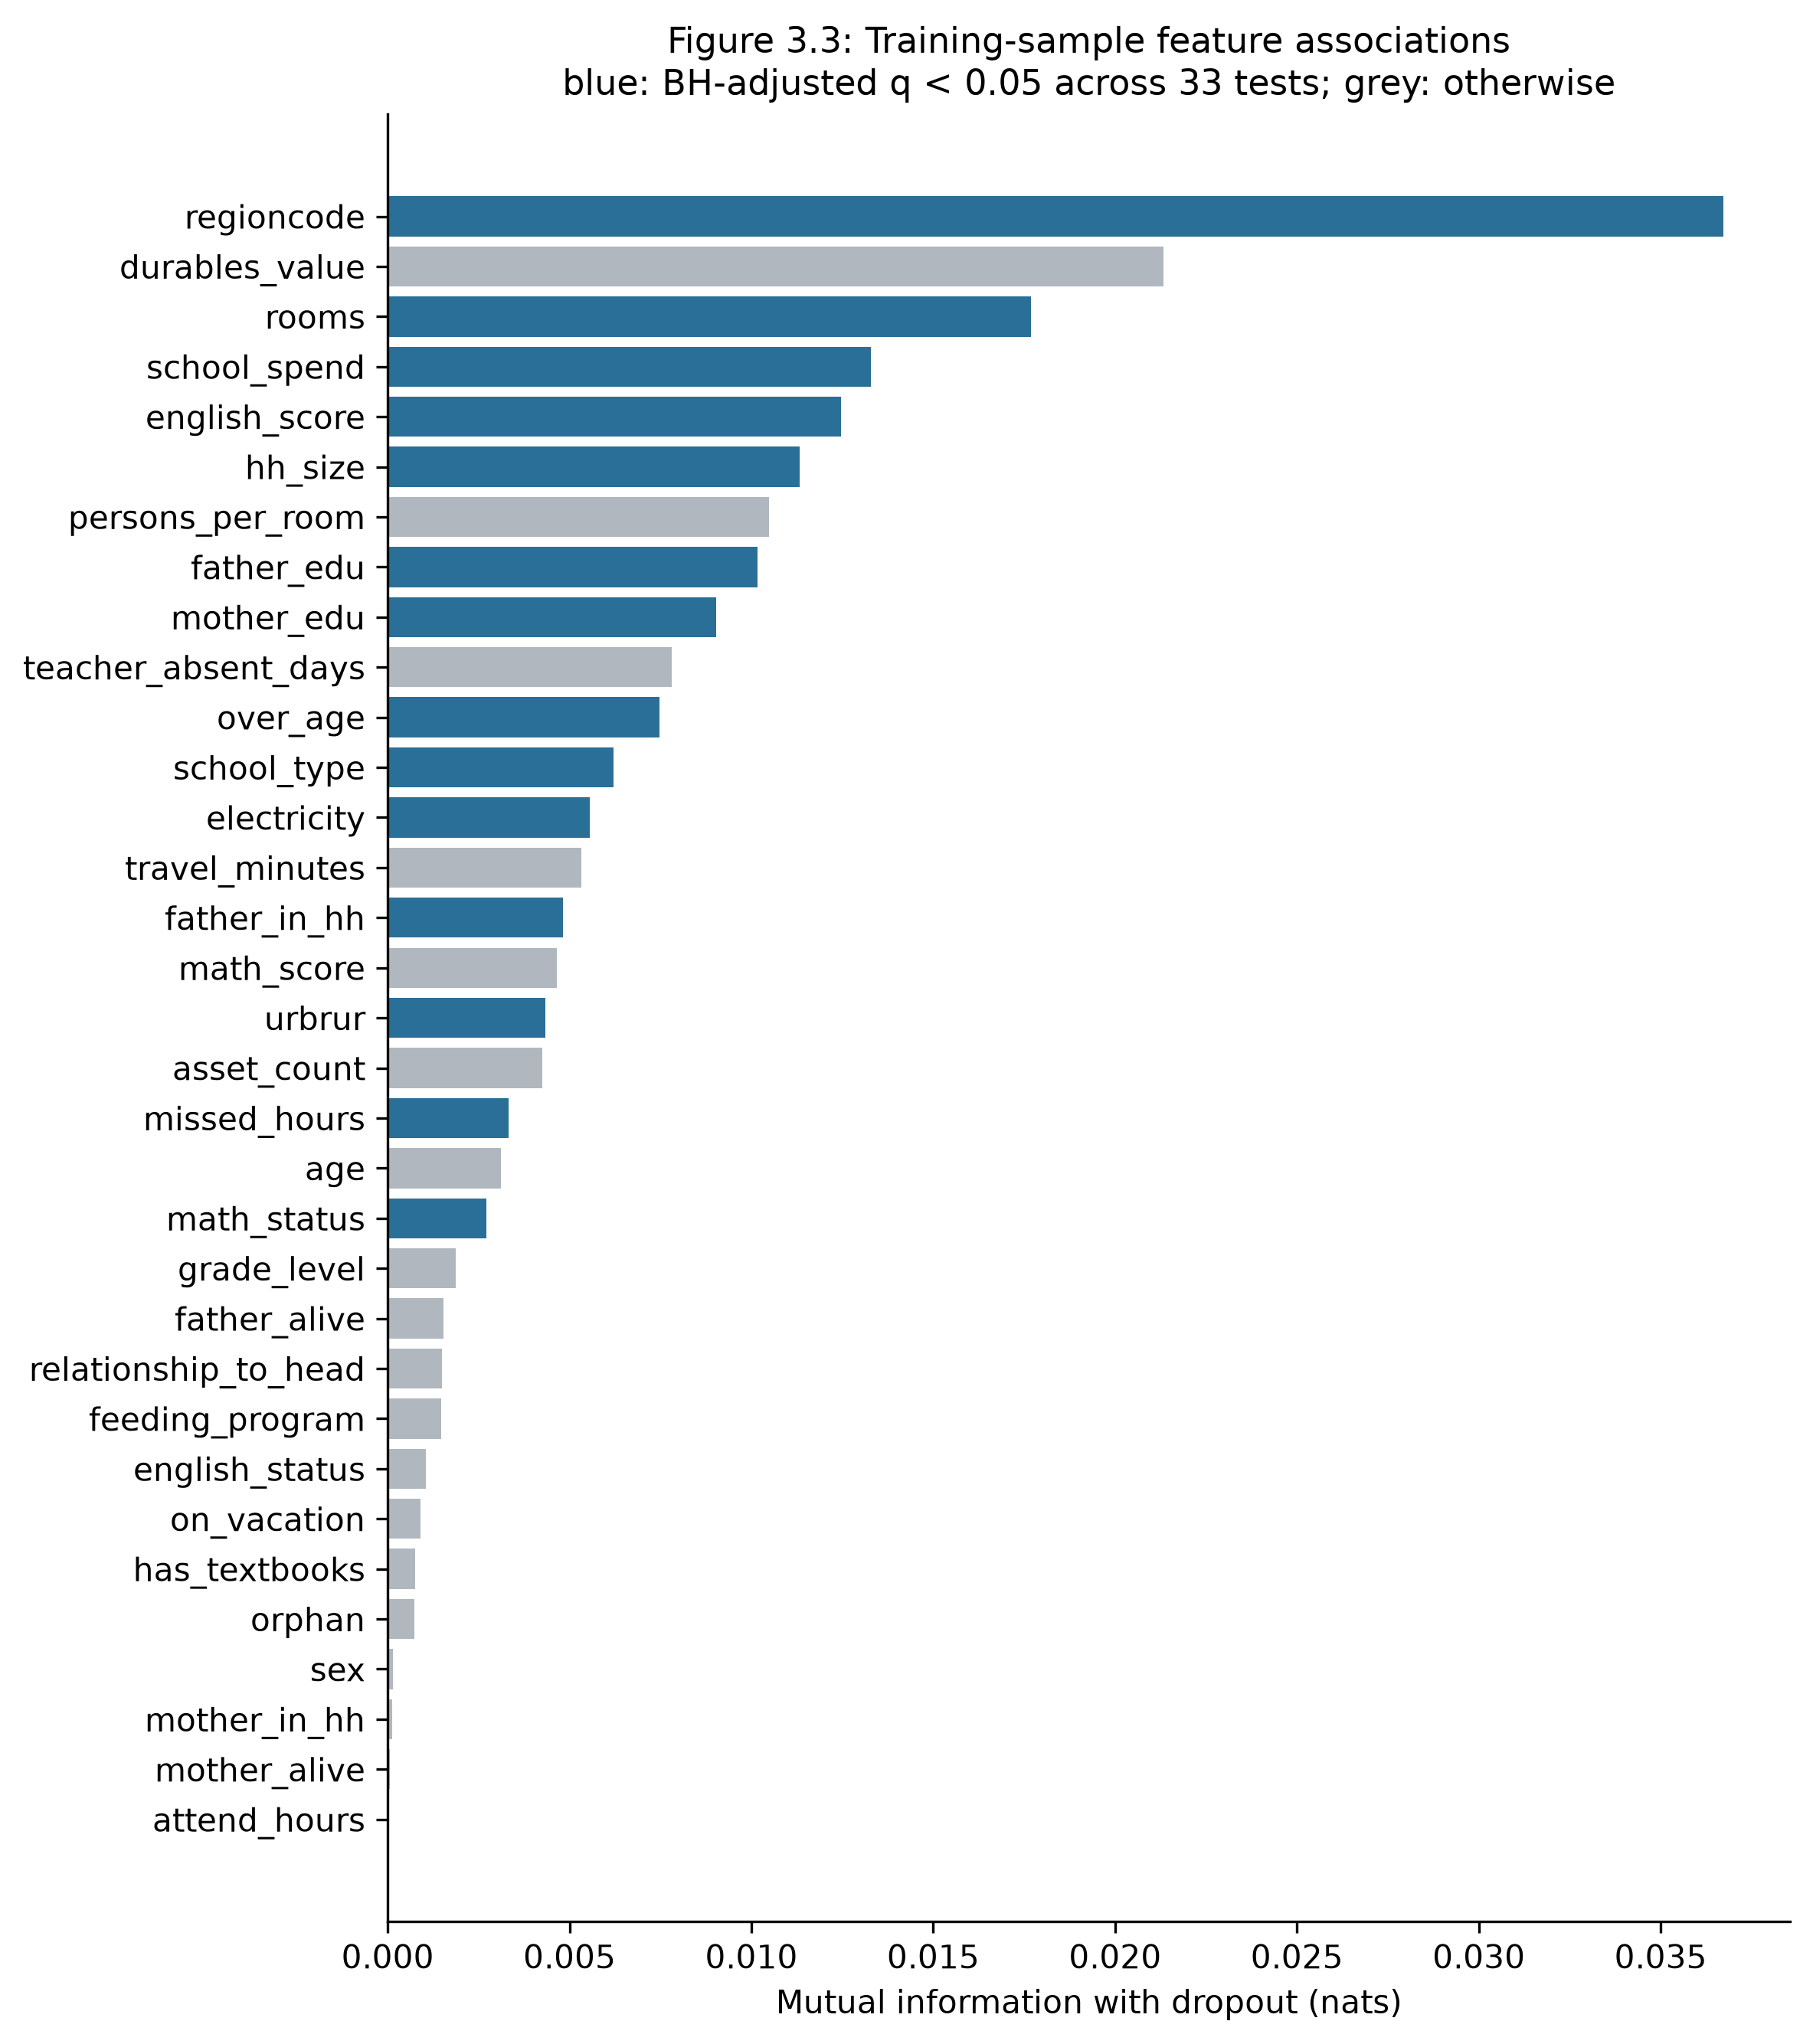
\includegraphics[width=0.85\columnwidth]{fig3_3_target_importance.png}
\caption{Which features tell us most about dropout. \emph{How to read it:} the longer the bar, the more knowing that feature helps to tell dropouts from children who stay (mutual information). Blue bars meet BH-adjusted $q<0.05$ across 33 exploratory tests; grey bars do not. This is not a causal or population inference. Region is at the top, followed by household and school-spending measures, test scores and parents' education.}
\label{fig:importance}
\end{figure}

\begin{figure}[!t]
\renewcommand{\thefigure}{3.1}
\centering
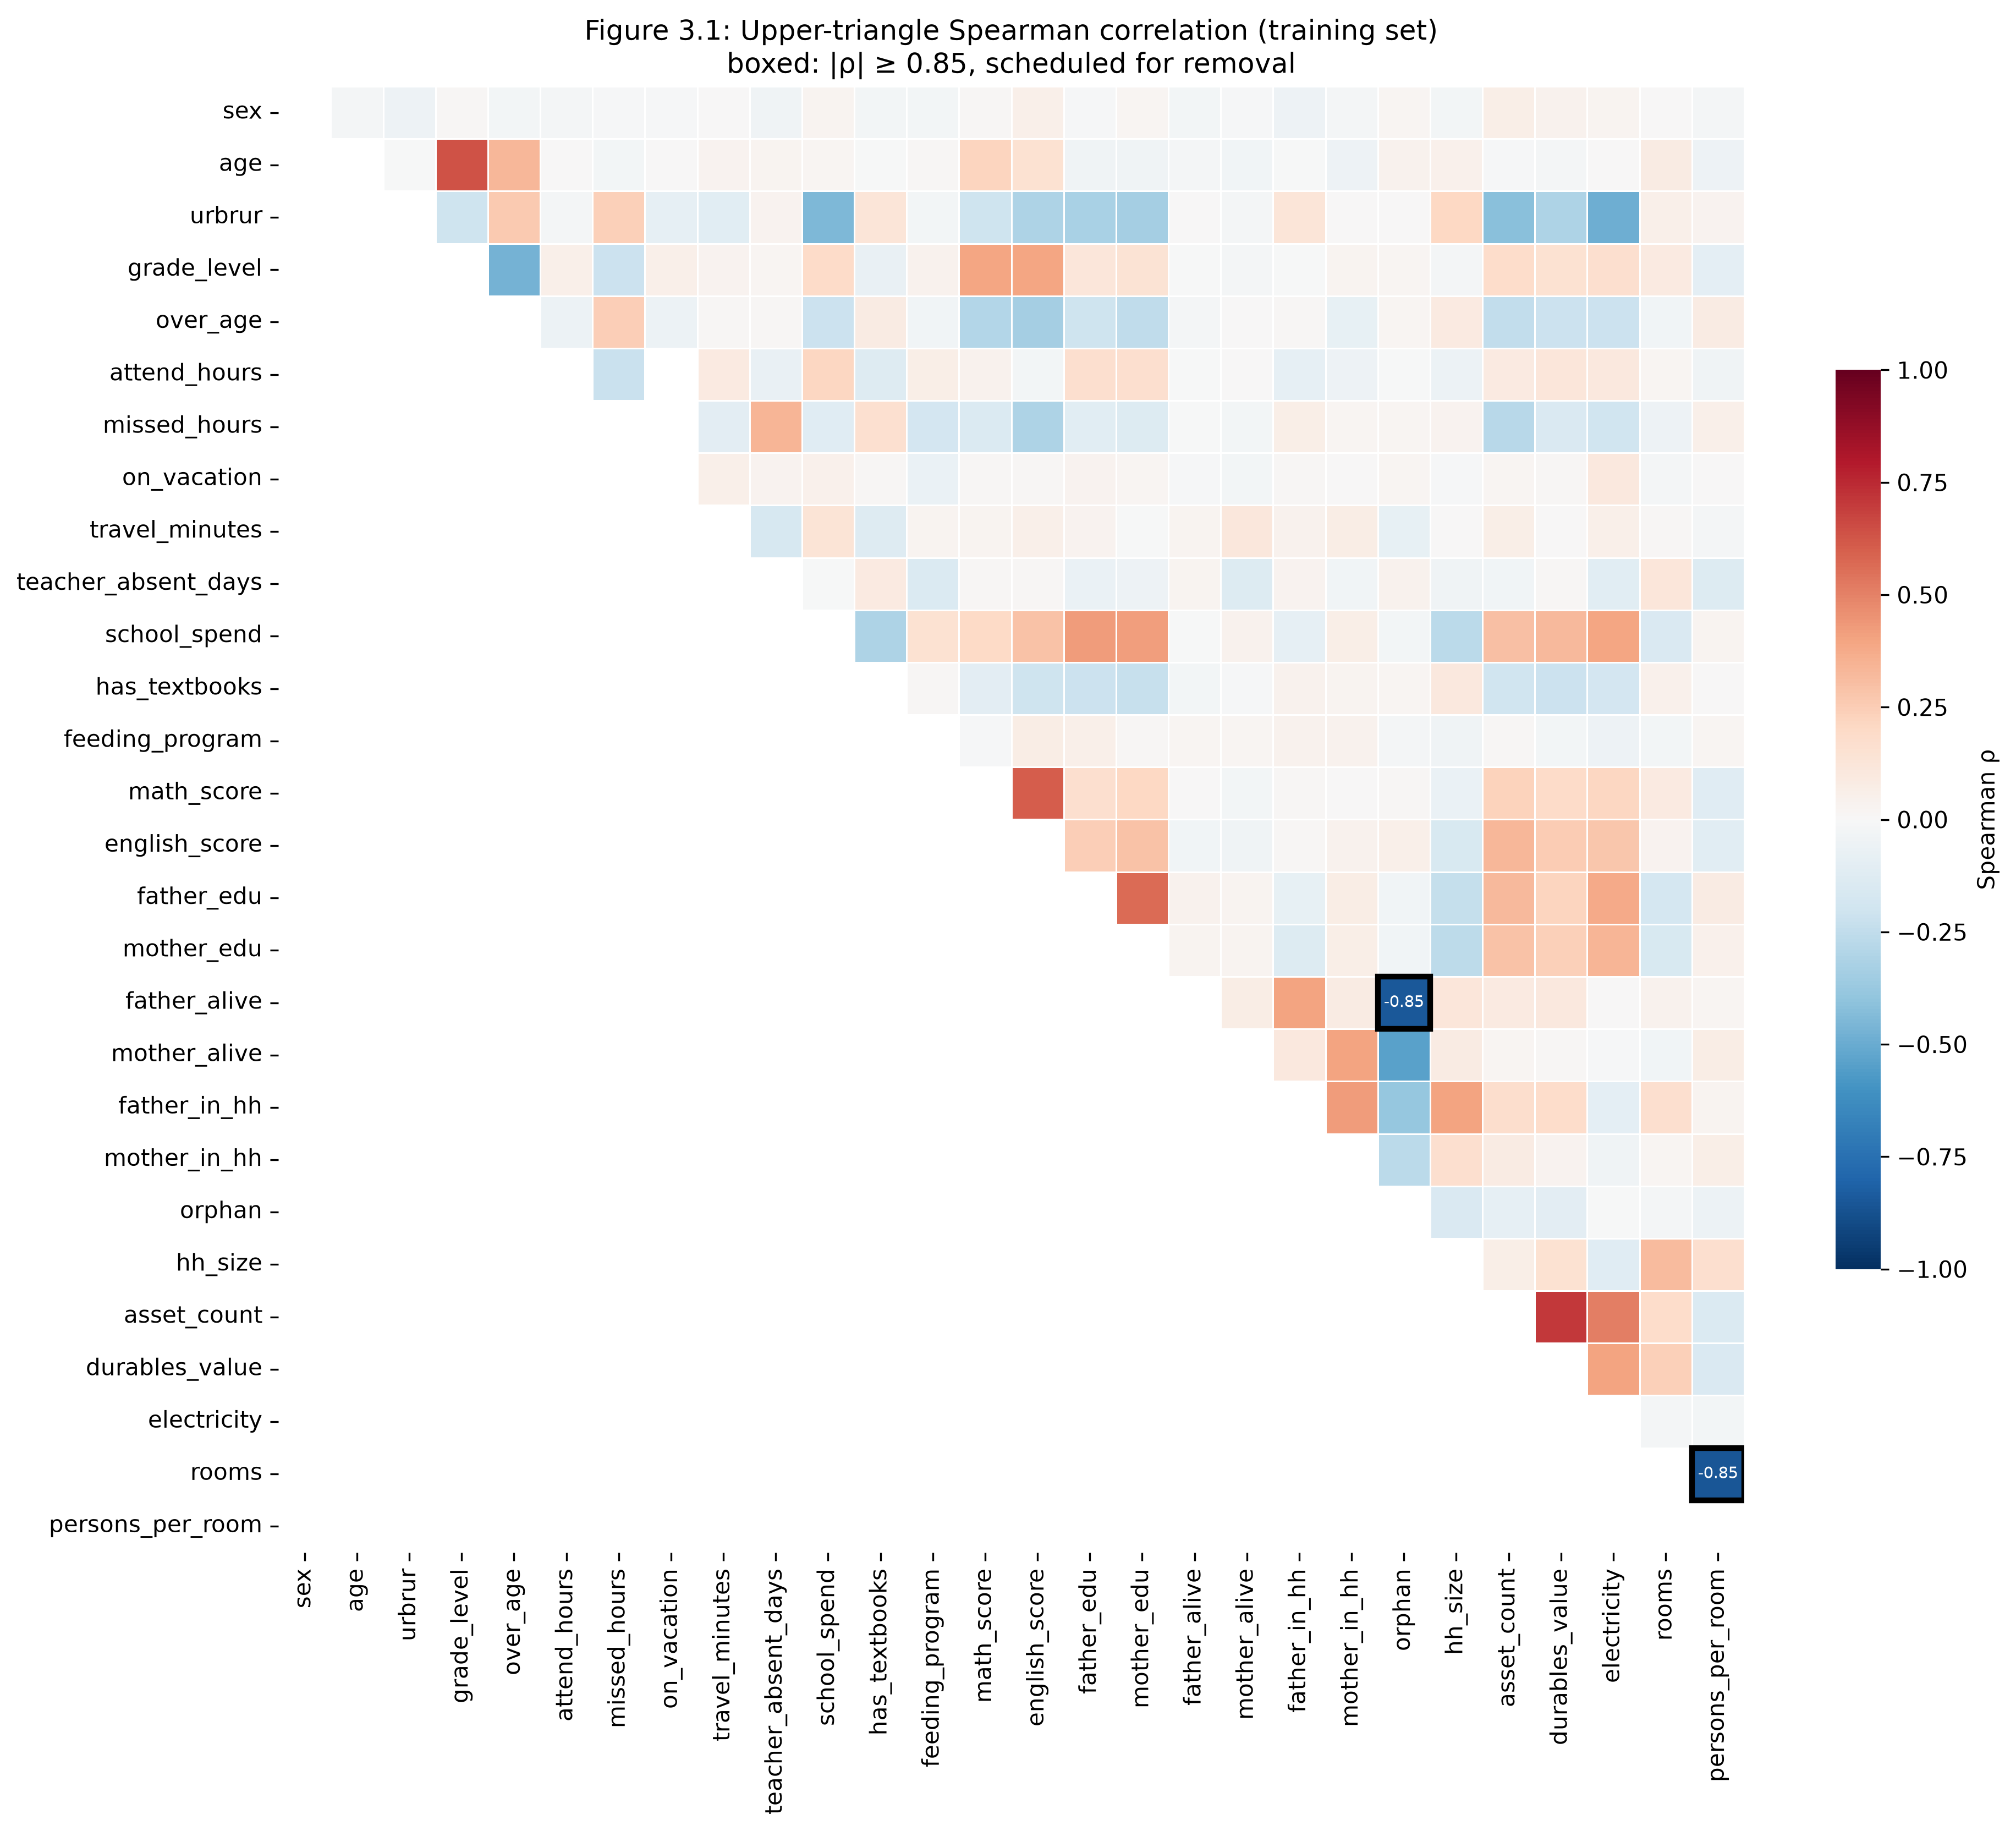
\includegraphics[width=0.9\columnwidth]{fig3_1_correlation_matrix.png}
\caption{Which features repeat each other. \emph{How to read it:} each small square compares two features (names on the left and bottom). Dark red: the two rise and fall together; dark blue: when one rises the other falls; white: no relationship. Only half of the grid is drawn because the other half is its mirror image. Boxed squares mark pairs so close (0.85 or more, ignoring the sign) that keeping both would repeat the same information; one of each pair is removed (Table~\ref{tab:b4b}).}
\label{fig:corr}
\end{figure}

\textbf{What this shows.} Region has the largest training-sample MI, but observed regional dropout rates changed over time, so transportability is uncertain. Across the 33 tests, \textbf{14} meet BH $q<0.05$; \textbf{13} meet the more conservative BY sensitivity. Effect sizes, not significance labels alone, describe how strong the associations are. Hours missed has a relatively large rank effect among the 290 children with recorded values, but its missingness limits the interpretation. No weak-link feature is removed from this exploratory screen.

\subsection*{B4b. Removing features that repeat each other (multicollinearity)}
\begin{figure*}[!t]
\renewcommand{\thefigure}{3.2}
\centering
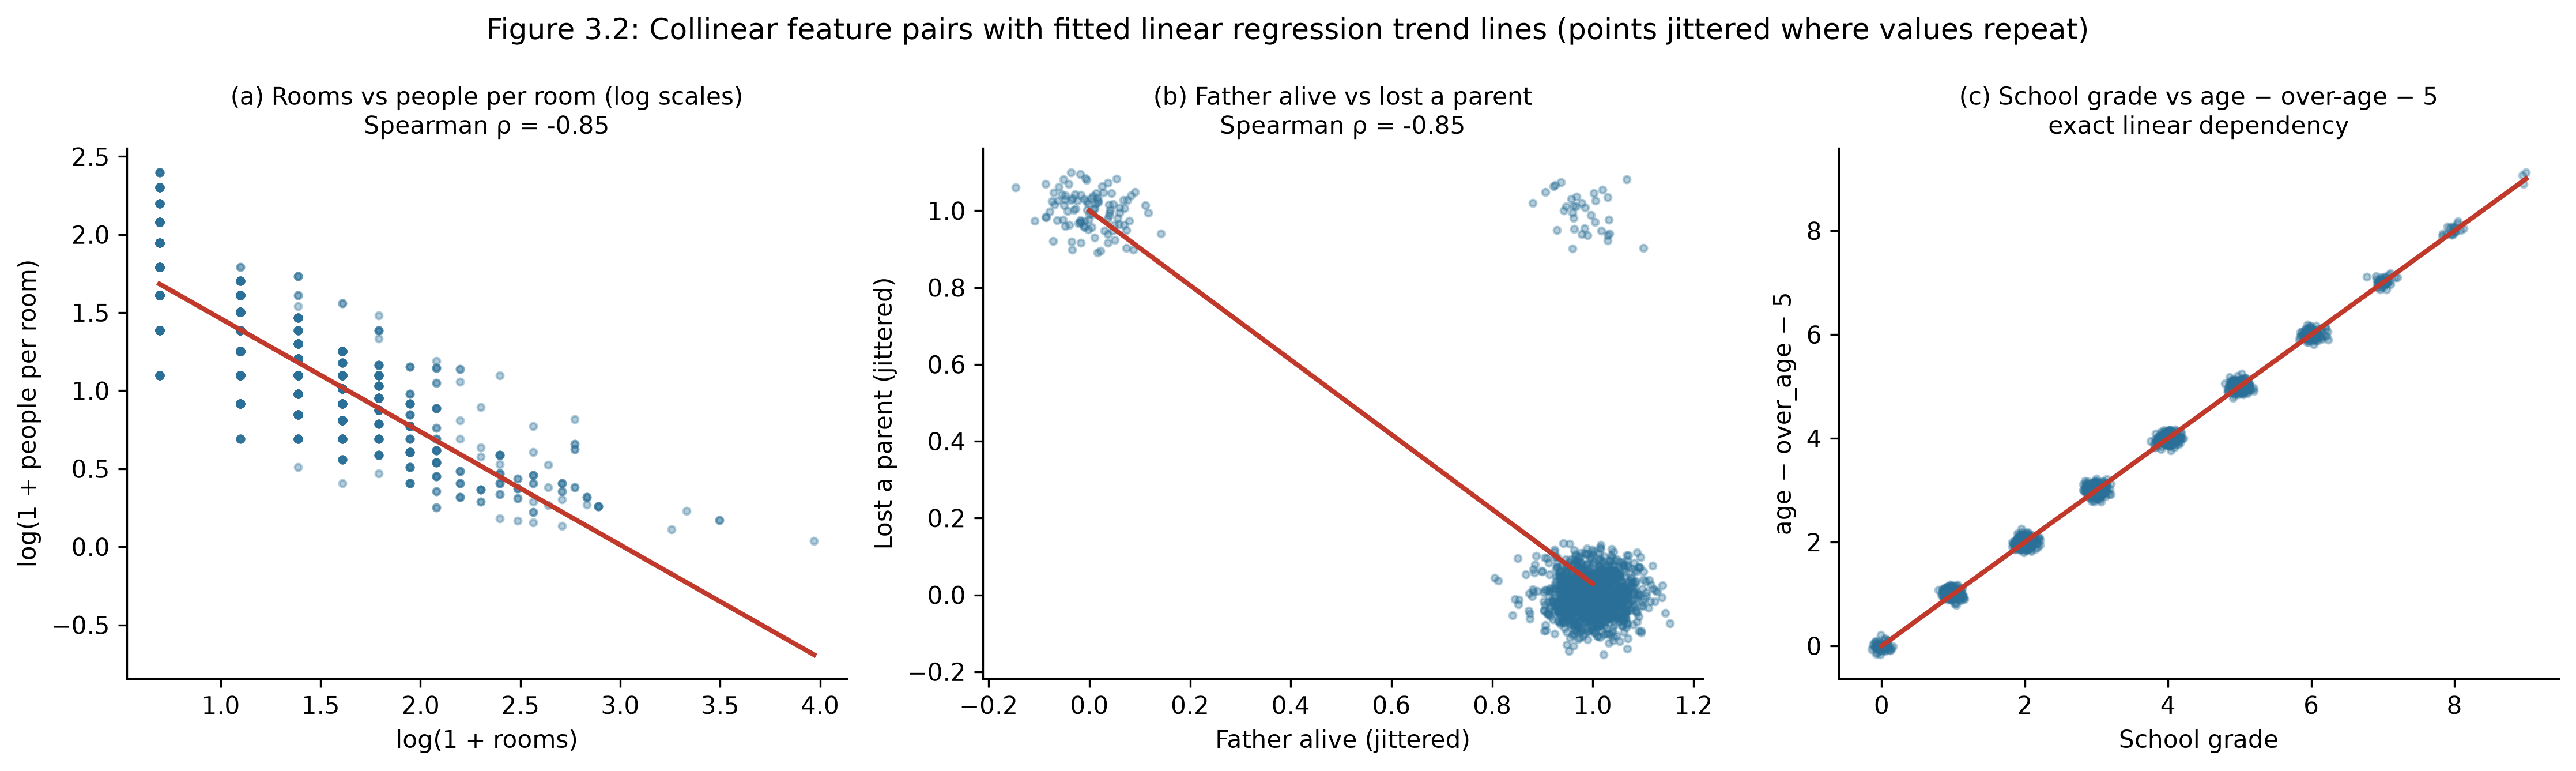
\includegraphics[width=0.92\textwidth]{fig3_2_collinear_scatterplots.png}
\caption{The three repeating features, one dot per child, with a straight line through the dots. (a) More rooms means fewer people per room (both on log scales, where the curve becomes almost a straight line), because people per room is calculated from rooms. (b) ``Lost a parent'' is almost exactly the opposite of ``father alive'' (dots are spread slightly so they do not sit on top of each other). (c) School grade can be calculated exactly from age and years over-age, so every dot lies on the line.}
\label{fig:collinear}
\end{figure*}

\textbf{Procedure.} (1) Compare every pair of features (Spearman correlation, which suits lopsided data) and flag pairs with $|\rho|\ge0.85$. (2) Check how much each feature is already explained by all the others together (VIF) and flag values above 10 \cite{obrien2007}. (3) \textbf{Fixed structural rule:} remove people per room and orphan status because their source items are retained. In the age--grade--over-age identity, retain age and the domain-relevant over-age signal, and remove grade. This decision does not depend on full-training target associations. (4) Re-check after removal. The result is in Table~\ref{tab:b4b} and Figs.~\ref{fig:corr}--\ref{fig:collinear}.

People per room has a low VIF (1.77) even though it closely follows rooms, because VIF only looks for straight-line overlap and this link is curved; the pair check, which works on rankings, catches it. The pair check finds the two calculated features; the VIF check finds the age, grade and over-age relationship that no single pair reveals (Fig.~\ref{fig:collinear}c). In theory school grade's VIF would be infinite (it is fully determined by age and over-age); it shows 19.9 only because its 81 missing values were filled with a typical value for this check. Removing these three features takes the count from 33 to 30 \textbf{without losing information}, since each one can be rebuilt from features that remain. Because the removal follows from how the features are built (each is calculated from others), the list of features to remove is fixed before cross-validation. For orphan status the derivation uses three-valued logic: either parent deceased gives 1, both alive gives 0, otherwise unknown. In the age, grade and over-age group any one can be calculated from the other two; grade is removed by the fixed domain rule above. An independent MI-only diagnostic agrees with the planned list in only \textbf{1 of 5 folds}; therefore the report does not claim that the information-based choice is stable. This diagnostic is descriptive and never changes the fixed list (\var{C2\_feature\_selection\_stability.csv}).

% ===============================================================
\section{Encoding, Scaling and Split Strategy (Part C)}
% ===============================================================
\begin{table*}[!t]
\centering
\caption{How each of the 30 remaining features is turned into numbers and rescaled (C1)}
\label{tab:c1}
\footnotesize
\begin{tabularx}{\textwidth}{L P{5.2cm} P{4.6cm}}
\toprule
Features & How it becomes numbers & Rescaling (simple model and PCA only) \\
\midrule
Region (10), school type (4 + missing), math and English test taken? (3) & One yes/no column per option & None (already 0/1) \\
Relationship to head & Grouped into 3 options, then one yes/no column each & None (already 0/1) \\
Father's and mother's education & Ordered numbers 0--4 & Common scale \\
Has textbooks & Ordered: none 0, some 1, all 2 & Common scale \\
Sex, urban/rural, holiday, feeding programme, parent items, electricity & 0 = no, 1 = yes & None (already 0/1) \\
Age, years over-age, hours attended, days teacher absent (75\% zeros, so not logged), scores, key assets & Kept as numbers & Common scale \\
Hours missed, travel time, household size, rooms & Kept as numbers & Log, then common scale \\
Value of household goods, school spending & Rank 0--1 against model-building values (after inflation adjustment) & Common scale \\
\bottomrule
\end{tabularx}
\tabnote{\emph{How to read it:} each row is a group of features. The middle column says how they become numbers; the last column says how they are rescaled for the simple model (logistic regression) and PCA. The main model, XGBoost, uses every feature \emph{without any rescaling}, because a decision tree only compares values (``is travel time above 45 minutes?''), so units do not matter (see text). Full table: \var{C1\_encoding\_scaling\_plan.csv}.}
\end{table*}

\begin{figure*}[!t]
\renewcommand{\thefigure}{4.1}
\centering
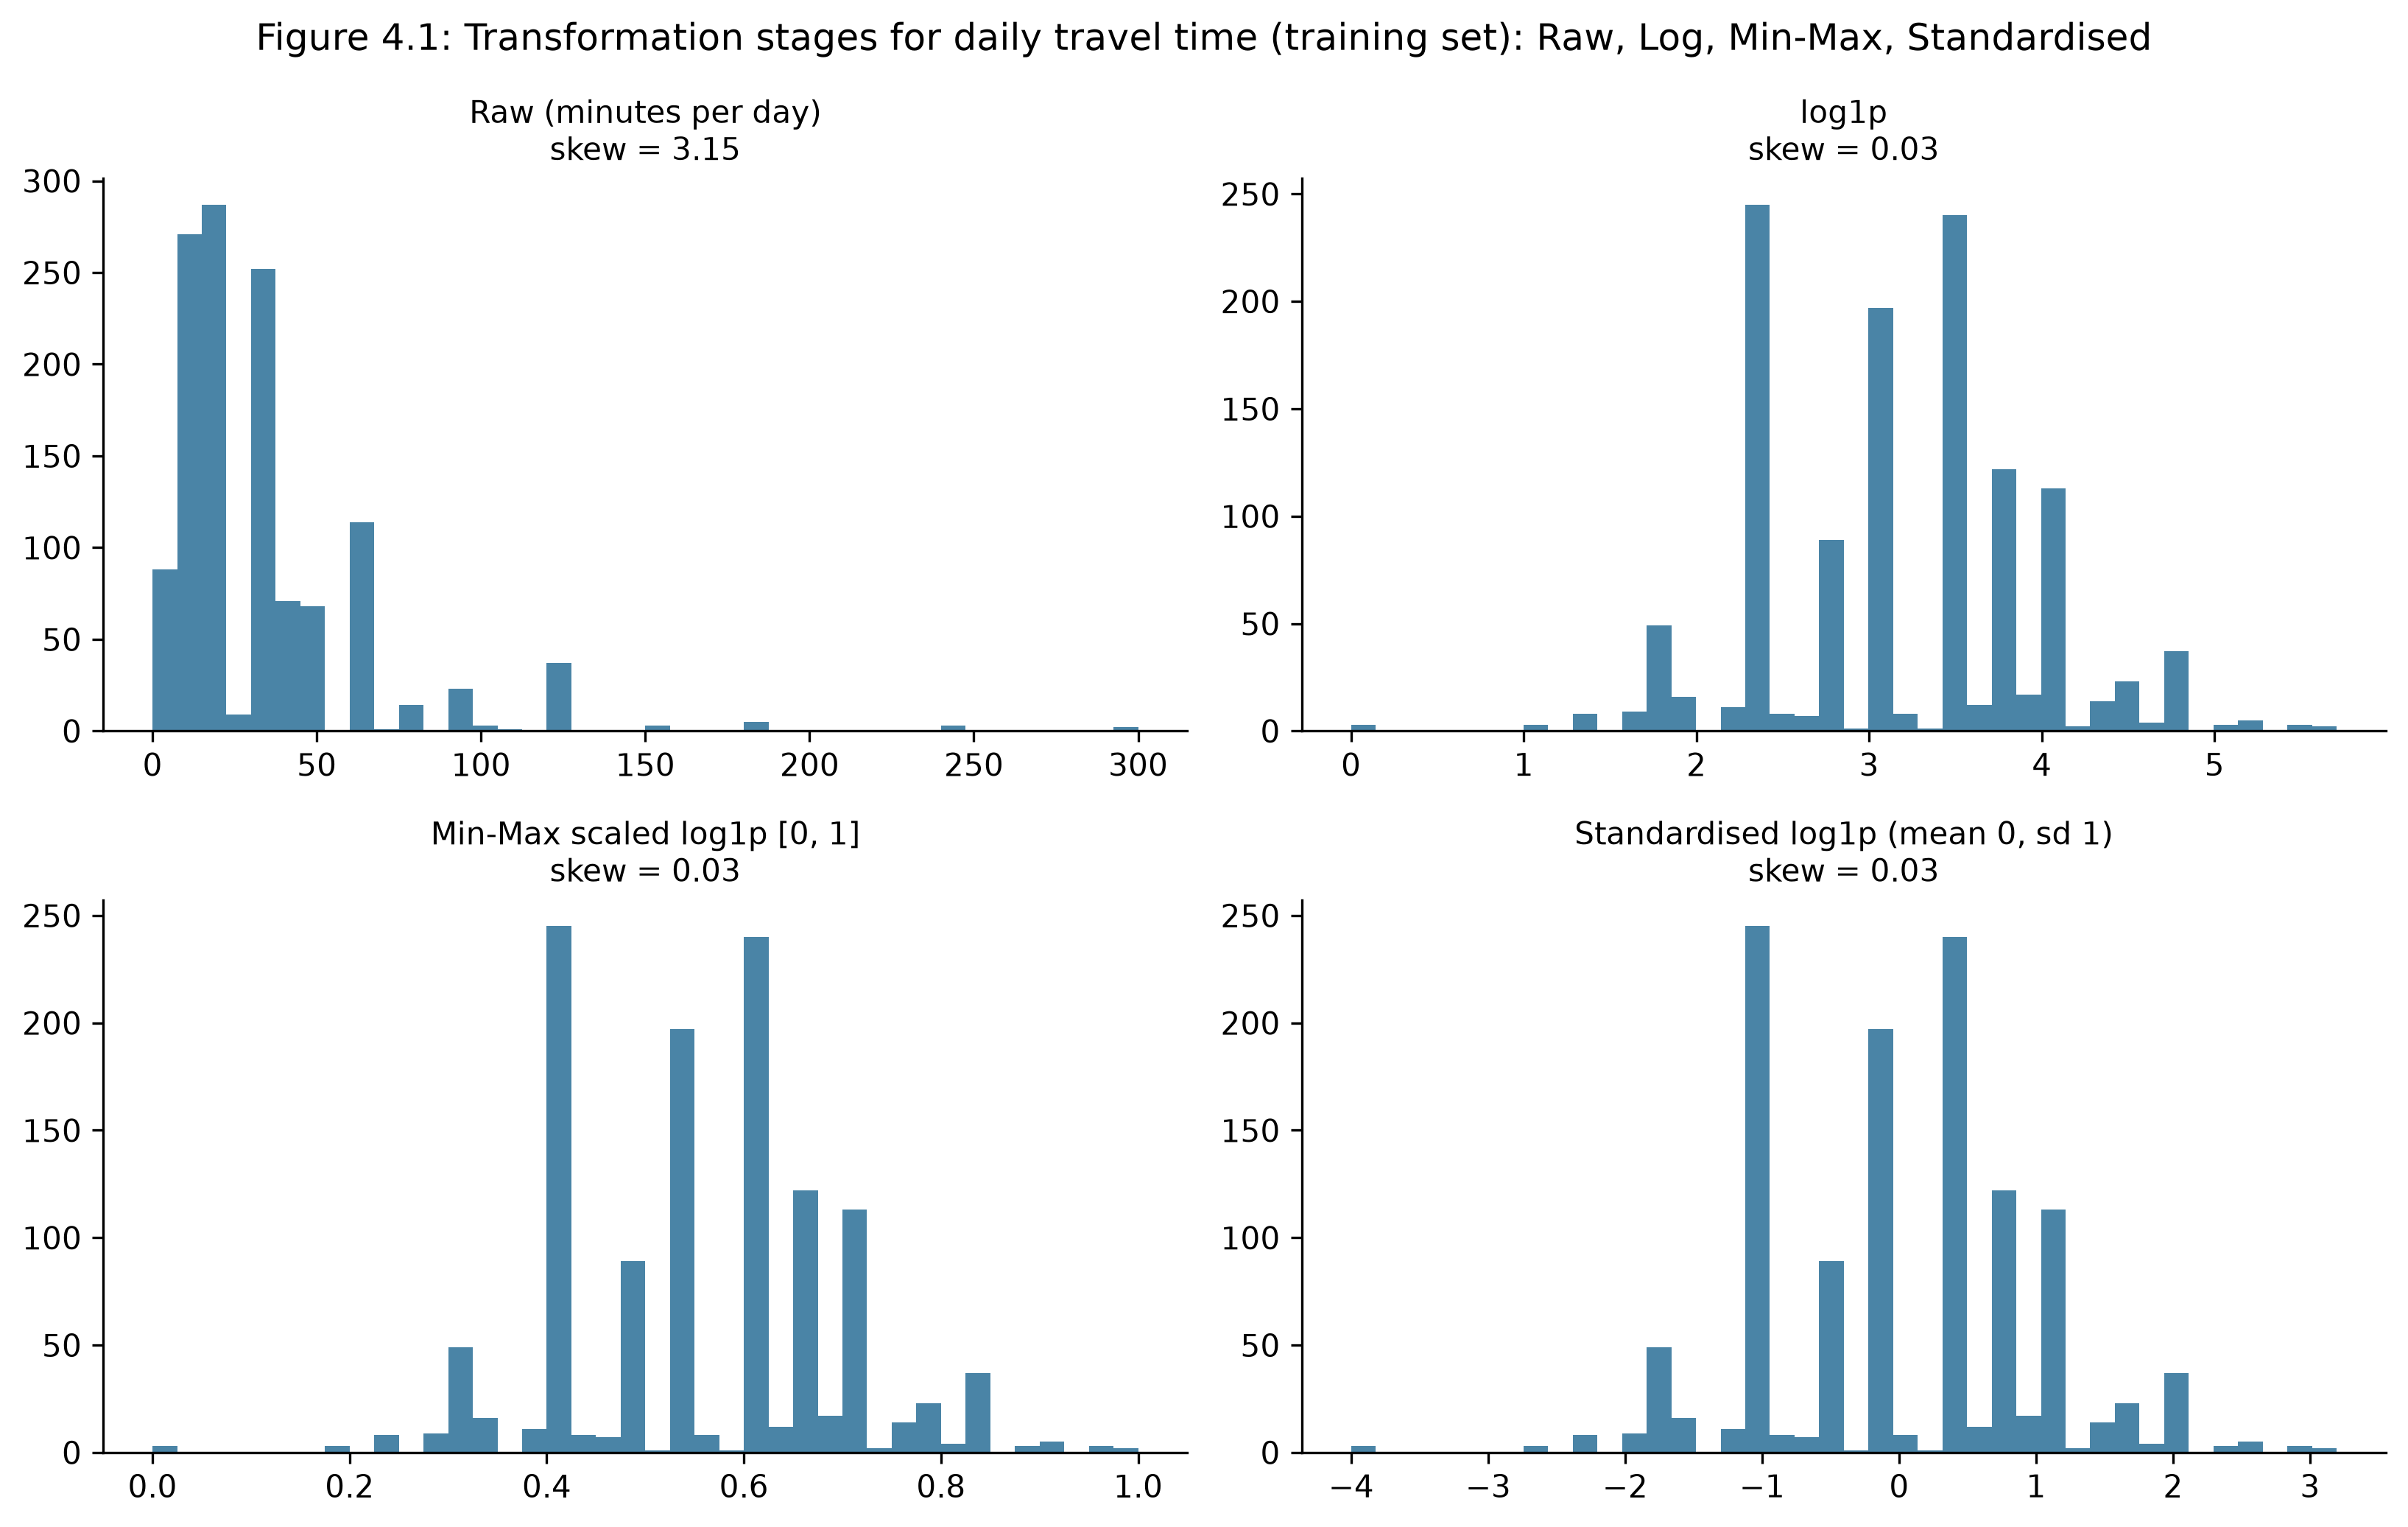
\includegraphics[width=0.8\textwidth]{fig4_1_transformation_grid.png}
\caption{What the preparation steps do to one feature, daily travel time. \emph{How to read it:} in each panel the height of a bar is the number of children with that value. \textbf{Top left (``Raw'')}: travel time as recorded; most children travel less than 50 minutes, but a few travel up to 300, which gives a long tail to the right (skew 3.15). \textbf{Top right (``log1p'')}: after the log transform the tail is pulled in and the shape becomes balanced (skew 0.03). \textbf{Bottom left}: the same values squeezed into 0--1 (Min--Max). \textbf{Bottom right}: the same values standardised (average 0, spread 1). The bottom two panels have exactly the same shape as the top right one; only the numbers on the bottom axis change. This is why the log is the step that matters and the last step only changes units. (The gaps between bars come from people rounding their travel time to 10, 15 or 30 minutes.)}
\label{fig:transform}
\end{figure*}

\subsection*{C1. Converting categories and putting numbers on a common scale}
\begin{table}[!t]
\centering
\caption{The five cross-validation folds (C2)}
\label{tab:folds}
\footnotesize
\setlength{\tabcolsep}{4pt}
\begin{tabular}{crrrrr}
\toprule
Fold & \makecell{Children\\to build} & \makecell{Children\\to check} & \makecell{Dropout \%\\(build)} & \makecell{Dropout \%\\(check)} & \makecell{Dropouts\\in check} \\
\midrule
1 & 1,042 & 265 & 14.4 & 14.3 & 38 \\
2 & 1,055 & 252 & 14.6 & 13.5 & 34 \\
3 & 1,037 & 270 & 14.0 & 15.9 & 43 \\
4 & 1,050 & 257 & 14.7 & 13.2 & 34 \\
5 & 1,044 & 263 & 14.3 & 14.8 & 39 \\
\bottomrule
\end{tabular}
\tabnote{The dropout share stays close to 14\% in every part (stratification). Checked for every fold: 0 districts and 0 households appear in both the building and the checking part, so related children are never split (grouping). Full table: \var{C2\_cv\_folds.csv}.}
\end{table}

\textbf{Categories into numbers (encoding).} Labels with no order (region, school type, relationship to head, test taken?) have at most 10 options, so each option becomes its own yes/no column (\emph{one-hot encoding}); this adds few columns and does not pretend one option is ``bigger'' than another. Relationship to head is first grouped into three options (own child 84\%, grandchild, other) because the rare options are too small to learn from. Ordered categories (parents' education and textbooks; school grade is removed in B4b) are turned into ordered numbers 0, 1, 2\ldots{} (lowest = 0; e.g.\ education: none 0, primary 1, middle/JSS 2, secondary 3, post-secondary 4), which keeps their order without adding any columns (\emph{ordinal encoding}); ``has textbooks'' is re-numbered so that a higher number means more books. Yes/no items become 0/1. A more complex method (target encoding) is not needed and would risk leakage with only 1,307 children.

\textbf{Money and inflation.} The two money features are long-tailed in training, so a training-reference rank bounds their influence to 0--1 without learning the later distribution. This is a project-specific robust transformation, not a claim that the cited asset-index literature prescribes it. Retain the fixed external CPI conversion to align monetary units before applying the stored training reference. The previously inspected difference between later and earlier household-goods medians (1,038 vs 405 cedis) is descriptive; it does not establish that inflation is the main cause. Wealth, prices, composition and measurement can all contribute. A later-wave within-wave rank would fit the test distribution, so it is not the primary evaluation procedure.

\textbf{Common scale (scaling).} The main model, XGBoost, is built from decision trees that only ask questions such as ``is travel time above 45 minutes?''. The answer depends only on the \emph{order} of values, so changing the units changes nothing, and \textbf{no rescaling is needed}. The simpler comparison model (regularised logistic regression, which shrinks every feature's effect by the same rule, so features on bigger scales would be treated unfairly) and the dimension-reduction summary planned for Phase 2 (PCA) combine the numbers directly, so features with large values (e.g.\ minutes of travel) would swamp features with small ones (e.g.\ a 0--7 score). For these, features with a long tail of high values are first log-transformed (except days teacher absent, where 75\% of values are 0) and then the 16 numeric/ordinal columns are put on a common scale (\emph{standardised} with scikit-learn's \var{StandardScaler}: average 0, spread 1). StandardScaler does not require Gaussian predictors: it changes centre and scale, not distribution shape. The log is a separate choice to compress long tails; scaling then aligns units for regularisation and PCA (Fig.~\ref{fig:transform}) \cite{standardscaler}. Standardising is preferred over squeezing values into 0--1 (\var{MinMaxScaler}), because Min--Max is thrown off by extreme values and none of our models (no neural network) requires a 0--1 range. The two money ranks are already bounded between 0 and 1; for the simple model they are standardised like the other numbers to align the numeric/ordinal units. The 32 remaining binary, one-hot and missingness-indicator columns of the 48-column LR/PCA matrix stay on their 0/1 scales. PCA centres this mixed-scaled matrix without additional standardisation; its variance shares are conditional on that choice. The full plan is in Table~\ref{tab:c1}, and Fig.~\ref{fig:transform} shows the steps on one feature.

\textbf{Final width:} 25 single columns (16 numbers or ordered numbers + 9 yes/no items) + 24 yes/no columns from the label options + 4 ``was missing'' flags (B1) = \textbf{53 columns} for XGBoost; 48 for logistic regression (one option per label is left out as the reference).

\subsection*{C2. Splitting the data and preventing leakage}
\begin{table*}[!t]
\centering
\caption{Summary of planned decisions (to be checked against what is built in Phase 2)}
\label{tab:summary}
\footnotesize
\renewcommand{\arraystretch}{1.0}
\begin{tabularx}{\textwidth}{P{3.4cm} L P{4.6cm}}
\toprule
Step & Planned decision & Learned from \\
\midrule
Fix recording errors & Special codes and impossible values $\rightarrow$ missing; travel-time box fix; survey-coded holiday vs inferred no-class proxy distinguished & Nothing (fixed rules) \\
Fill gaps (B1) & Average if balanced, middle value if lopsided; most common answer for yes/no and ordered items; mixed-distance KNN with k selected inside each fit for grade; ``missing'' option for school type; 4 ``was missing'' flags (teacher absent, hours attended, father's and mother's education); blank hours missed assumed 0 (sensitivity check) & Building part of each fold \\
Extreme values (B2--B3) & IQR rule on the log scale (no feature is bell-shaped); cap the high end (13 values), delete nobody; key warning signs and fixed scales not capped; money features ranked instead & Building part of each fold \\
Links to dropout (B4a) & Mann--Whitney, chi-square and mutual information, each matched to the feature type & Model-building table \\
Repeating features (B4b) & Correlation $\ge0.85$ or VIF $>10$; remove people per room, lost a parent, school grade (33 $\rightarrow$ 30), all exact calculations from kept features; removed inside each fold after gaps are filled & Fixed structural/domain rule, independent of target; MI-only stability reported separately \\
Categories to numbers (C1) & Yes/no column per option (up to 10 options), ordered numbers, 0/1, money converted to 2009/10 prices and ranked (53 columns) & Building part of each fold \\
Common scale (C1) & Not needed for XGBoost; log then standardise for the simple model and PCA & Building part of each fold \\
Fewer dropouts (A4) & Extra weight on dropouts ($\approx$6$\times$); judged by PR-AUC and dropouts caught in the top 20\% & Building part of each fold \\
Splitting (C2) & Primary: later, novel households (731 children); secondary: new people (1,175); five district-grouped training folds; previously explored temporal data disclosed & Nothing (fixed design) \\
\bottomrule
\end{tabularx}
\end{table*}

\textbf{(a) Allocation.} The full linked inputs remain 1,307 training children (Wave 1 to 2) and 1,395 later children (Wave 2 to 3): 48\%/52\% before entity exclusions. The \textbf{primary temporal evaluation} uses only children from households absent from training: \textbf{731} children, \textbf{76} dropouts, \textbf{605} households. With 1,307 training rows this is an effective \textbf{64.1\%/35.9\%} allocation. No household or person is shared with training. The \textbf{secondary temporal evaluation} excludes repeated people but permits known households: 1,175 children, 115 dropouts, 370 shared households. The full 1,395-row cohort is descriptive only. Cohort definitions use household/person IDs, never outcomes (\var{C2\_temporal\_cohorts.csv}).

\textbf{(b) Training validation.} Use five \var{StratifiedGroupKFold} folds with whole districts, shuffle enabled and seed 42. Their validation shares are about 20\%, with 34--43 dropouts per fold; there is no shared district or household within a fold. Exact fold sizes and class shares are in Table~\ref{tab:folds}. A random 70/15/15 split would leave only about 28 dropouts in each small partition. The temporal cohorts are fixed by time and IDs, so they are not forcibly stratified to match training.

\textbf{(c) Fit boundaries.} Fit every imputer, cap, encoder, rank reference and scaler on the building rows only. Grade KNN chooses its neighbour count in three additional district-grouped inner folds of that fit, using grade recovery rather than dropout. Structural feature removals are fixed, independent of full-training target associations. During later model tuning, use inner training folds to select settings, calibration and thresholds; assess only on the outer checking fold, then refit the frozen procedure on all training children.

\textbf{(d) What the temporal test can claim.} Later-period covariates, dropout rates and regional summaries have already been inspected during development. This cannot be undone: the temporal cohort is a \textbf{retrospective, previously explored evaluation}, not an untouched confirmatory holdout. The implemented numerical fitting and KNN selection use training only. Freeze the procedure before computing primary and secondary prediction metrics, and do not choose models from those temporal scores. A genuinely unseen future or external cohort is needed for confirmation. Shared districts remain across time; primary separation is by household, not a claim of transport to new districts.

\textbf{(e) Reproducibility and checks.} The identity masks, effective allocations and raw-data SHA-256 values are recorded in \var{C2\_evaluation\_protocol.json}. The primary mask must have zero shared people and households; the secondary mask must have zero shared people. Transforming either temporal subset must leave fitted pipeline settings unchanged. The model inputs remain 53 columns for XGBoost or 48 for logistic regression; cohort flags are metadata, never predictors.

% ===============================================================
\section{Changes over Time and Limitations}
\label{sec:limits}
% ===============================================================
\begin{itemize}
\item \textbf{Children who could not be found again (selection-bias risk).} Their observed characteristics differ (older, less often living with parents), creating selection-bias risk; the missingness mechanism and direction of dropout-rate bias remain unknown. The 164 children rejected by the identity check are also poorer and more rural; allowing an age change of 1--8 years would add 59 children (13 of whom left school); this is tested as a sensitivity check.
\item \textbf{The situation changed between periods.} Dropout fell from 14.4\% to 10.4\% overall, from 28\% to 12\% in the Northern region and from 46\% to 12\% in Upper West. What the model learns about regions may not carry over, and its risk percentages may overstate later risk.
\item \textbf{Different ways of collecting data.} Paper forms (2009/10) and tablets (2013/14) leave different gaps (e.g.\ hours missed: 77.8\% vs 11.7\% missing), and the 2013/14 tests added a fifth answer option (``none of the above''), so scores are not perfectly comparable. A ``was missing'' flag can therefore mean different things in the two periods, so a rule replaces a flag where possible (e.g.\ blank hours missed = 0, Table~\ref{tab:b1}); the effect of the four kept flags will be compared between periods in Phase 2.
\item \textbf{Change from the proposal.} Household consumption totals exist only for 2009/10, so wealth is measured in both periods by key assets, value of household goods, electricity, rooms and household size.
\item \textbf{Links, not causes.} The tests show which features go together with dropout, which is what prediction needs; they do not show that these features cause dropout.
\end{itemize}

% ===============================================================
\section{Summary of Planned Decisions}
% ===============================================================
Table~\ref{tab:summary} lists every planned decision and the data each step may look at, to be checked against Phase 2.

% ===============================================================
\FloatBarrier
\section*{Appendix: Plain-Language Guide to the Technical Terms}
\label{app:glossary}
The assignment requires several technical terms. Each is explained below in plain words.

{\footnotesize
\noindent\textbf{Feature:} One piece of information about a child, e.g.\ age or hours of class missed.\par\vspace{2pt}
\noindent\textbf{Target ($Y$):} What we want to predict: dropped out (1) or still in school (0).\par\vspace{2pt}
\noindent\textbf{Model-building table (training data) / testing table (test data):} Children used to build the model / children kept aside to check it honestly afterwards. The \emph{building part} and \emph{checking part} are the two pieces of the model-building table in each round of cross-validation.\par\vspace{2pt}
\noindent\textbf{Cross-validation (CV), fold:} Splitting the training data into 5 parts (``folds''); the model is built on 4 and checked on the 5th, rotating 5 times.\par\vspace{2pt}
\noindent\textbf{Leakage:} When information from the data used for checking sneaks into building the model, making results look better than they really are.\par\vspace{2pt}
\noindent\textbf{MCAR / MAR / MNAR:} Three reasons data go missing. \emph{MCAR}: by pure chance; \emph{MAR}: for a reason we can see in other answers (e.g.\ younger children were not tested); \emph{MNAR}: because of the hidden value itself (e.g.\ a child who cannot read leaves the reading test blank).\par\vspace{2pt}
\noindent\textbf{Imputation:} Filling a missing value with a sensible estimate.\par\vspace{2pt}
\noindent\textbf{Mean / median / mode:} The average / the middle value / the most common answer.\par\vspace{2pt}
\noindent\textbf{Typical value:} The middle value (median): half of the children are below it, half above.\par\vspace{2pt}
\noindent\textbf{Skewness (skew):} How lopsided a distribution is. Near 0 = balanced; large = a long tail of very high values (e.g.\ a few very rich households).\par\vspace{2pt}
\noindent\textbf{Outlier; IQR rule; Z-score rule:} An unusually extreme value; two standard rules for spotting one: the \emph{IQR rule} flags values far outside the middle half of the data, the \emph{Z-score rule} flags values more than 3 standard deviations from the average (a Gaussian tail interpretation needs a bell shape).\par\vspace{2pt}
\noindent\textbf{Capping (Winsorising):} Pulling an extreme value back to a set limit instead of deleting the child.\par\vspace{2pt}
\noindent\textbf{Log transform (log1p):} A standard way to compress a long tail so that very large values no longer dominate.\par\vspace{2pt}
\noindent\textbf{$p$-value; adjusted $q$:} A $p$-value is a tail probability under a no-association model, not the probability that the model is true. BH/BY adjust a family for multiple comparisons; a flagged adjusted value remains exploratory here.\par\vspace{2pt}
\noindent\textbf{Effect size (``strength of link'' in the tables):} How \emph{strong} a link is (0 = none, larger = stronger), regardless of sample size. Two are used: \emph{rank-biserial $r$} for numbers ($-1$ to $+1$; the sign says whether dropouts have higher or lower values) and \emph{Cram\'er's $V$} for categories (0 to 1).\par\vspace{2pt}
\noindent\textbf{Mann--Whitney test; chi-square test:} Two standard tests of whether dropouts differ from children who stayed. \emph{Mann--Whitney}: lines all children up from lowest to highest value and checks whether dropouts sit higher or lower in the line. \emph{Chi-square}: checks whether the dropout rate differs between groups (e.g.\ urban vs rural).\par\vspace{2pt}
\noindent\textbf{Mutual information (MI):} How much knowing a feature reduces uncertainty about dropout; captures any kind of relationship.\par\vspace{2pt}
\noindent\textbf{Correlation ($\rho$); VIF:} How closely two features move together ($-1$ to $+1$); VIF (variance inflation factor) shows how much a feature is already explained by all the others together (above 10 = redundant).\par\vspace{2pt}
\noindent\textbf{One-hot encoding:} Turning a category with several options (e.g.\ 10 regions) into separate yes/no columns.\par\vspace{2pt}
\noindent\textbf{Scaling (standardising):} Putting numbers measured in different units (cedis, hours, years) on a common scale.\par\vspace{2pt}
\noindent\textbf{XGBoost; logistic regression:} The main prediction model (built from many decision trees); a simpler baseline model used for comparison.\par\vspace{2pt}
\noindent\textbf{PR-AUC:} A score from 0 to 1 for how well the model puts real dropouts at the top of its risk list; it is the right score when dropouts are rare.\par\vspace{2pt}
\noindent\textbf{PCA:} A method that summarises many features into a few combined ones; planned for Phase 2.\par\vspace{2pt}
\noindent\textbf{KNN (nearest neighbours):} Filling a missing grade from children similar in age, sex, urban/rural, region and assets. Numeric differences and category matches are treated separately. The neighbour count is selected using training-only grouped validation; the full-training fit selects 15.\par\vspace{2pt}
\noindent\textbf{Stratification; grouping:} Keeping dropout shares approximately balanced (13.2--15.9\% across validation folds here), subject to whole-district grouping; keeping related children (same household or district) together in one fold.\par\vspace{2pt}
\noindent\textbf{StratifiedGroupKFold; \var{X\_train}; Pipeline:} The scikit-learn tool that keeps whole districts together while approximately balancing dropout shares; the building part of the data; the container that re-learns every preparation step inside each fold.\par\vspace{2pt}
\noindent\textbf{Cedi; P3, JSS:} Ghana's currency; Primary year 3 and Junior Secondary School (the last three years of basic education).\par\vspace{2pt}
\noindent\textbf{Overfitting; statistical power:} A model learning quirks of its building data that do not repeat in new data; the ability of a study to detect a real link, which falls when there are fewer cases.\par\vspace{2pt}
\noindent\textbf{Class weighting:} Counting each dropout several times more during training so the model pays enough attention to the rare group (\var{scale\_pos\_weight} in XGBoost).\par\vspace{2pt}
\noindent\textbf{Calibration:} Adjusting risk scores so that ``20\% risk'' really means about 1 in 5 such children drop out.\par\vspace{2pt}
\noindent\textbf{D'Agostino--Pearson test:} A standard test of whether numbers follow a bell shape.\par\vspace{2pt}
\noindent\textbf{Target encoding:} Replacing each category with the dropout rate of that category; not used here because it can leak outcome information.\par\vspace{2pt}
\noindent\textbf{Regularised model:} A model that is penalised for relying too heavily on any one feature, which keeps it simple.\par\vspace{2pt}
\noindent\textbf{ColumnTransformer; fit / transform:} The scikit-learn tool that applies the right preparation to each group of columns; \emph{fit} = learn the settings (e.g.\ a median) from data, \emph{transform} = apply them.\par\vspace{2pt}
\noindent\textbf{TimeSeriesSplit:} A way of making folds that always checks on later time points; needed only when data have many time points.\par\vspace{2pt}
\noindent\textbf{Sensitivity check:} Repeating an analysis with a different reasonable choice to see whether the conclusion changes.\par\vspace{2pt}
\noindent\textbf{Consumer price index:} The official measure of how prices rise over time, used to convert money to the prices of one year.\par\vspace{2pt}
}


% ===============================================================
\clearpage
\begin{thebibliography}{99}
\bibitem{balfanz2007} R.~Balfanz, L.~Herzog and D.~J. Mac~Iver, ``Preventing student disengagement and keeping students on the graduation path in urban middle-grades schools: Early identification and effective interventions,'' \emph{Educational Psychologist}, vol.~42, no.~4, pp.~223--235, 2007.
\bibitem{shap} S.~M. Lundberg and S.-I. Lee, ``A unified approach to interpreting model predictions,'' in \emph{Advances in Neural Information Processing Systems}, vol.~30, 2017, pp.~4765--4774.
\bibitem{gsps} Institute of Statistical, Social and Economic Research (University of Ghana), Economic Growth Center (Yale University) and Northwestern University, \emph{Ghana Socioeconomic Panel Survey, Waves 1--3} [Dataset], Harvard Dataverse, 2022, doi:10.7910/DVN/E5QP0F.
\bibitem{rubin1976} D.~B. Rubin, ``Inference and missing data,'' \emph{Biometrika}, vol.~63, no.~3, pp.~581--592, 1976.
\bibitem{littlerubin} R.~J.~A. Little and D.~B. Rubin, \emph{Statistical Analysis with Missing Data}, 3rd ed. Hoboken, NJ: Wiley, 2019.
\bibitem{tukey} J.~W. Tukey, \emph{Exploratory Data Analysis}. Reading, MA: Addison-Wesley, 1977.
\bibitem{kerby} D.~S. Kerby, ``The simple difference formula: An approach to teaching nonparametric correlation,'' \emph{Comprehensive Psychology}, vol.~3, 2014.
\bibitem{kraskov} A.~Kraskov, H.~St\"ogbauer and P.~Grassberger, ``Estimating mutual information,'' \emph{Physical Review E}, vol.~69, 066138, 2004.
\bibitem{ross2014} B.~C. Ross, ``Mutual information between discrete and continuous data sets,'' \emph{PLoS ONE}, vol.~9, no.~2, e87357, 2014.
\bibitem{obrien2007} R.~M. O'Brien, ``A caution regarding rules of thumb for variance inflation factors,'' \emph{Quality \& Quantity}, vol.~41, pp.~673--690, 2007.
\bibitem{filmer2001} D.~Filmer and L.~H. Pritchett, ``Estimating wealth effects without expenditure data---or tears: An application to educational enrollments in states of India,'' \emph{Demography}, vol.~38, no.~1, pp.~115--132, 2001.
\bibitem{saito2015} T.~Saito and M.~Rehmsmeier, ``The precision-recall plot is more informative than the ROC plot when evaluating binary classifiers on imbalanced datasets,'' \emph{PLoS ONE}, vol.~10, no.~3, e0118432, 2015.
\bibitem{xgboost} T.~Chen and C.~Guestrin, ``XGBoost: A scalable tree boosting system,'' in \emph{Proc. 22nd ACM SIGKDD}, 2016, pp.~785--794.
\bibitem{sklearn} F.~Pedregosa \emph{et al.}, ``Scikit-learn: Machine learning in Python,'' \emph{Journal of Machine Learning Research}, vol.~12, pp.~2825--2830, 2011.
\bibitem{zadrozny2002} B.~Zadrozny and C.~Elkan, ``Transforming classifier scores into accurate multiclass probability estimates,'' in \emph{Proc. 8th ACM SIGKDD}, 2002, pp.~694--699.
\bibitem{kaufman2012} S.~Kaufman, S.~Rosset, C.~Perlich and O.~Stitelman, ``Leakage in data mining: Formulation, detection, and avoidance,'' \emph{ACM Transactions on Knowledge Discovery from Data}, vol.~6, no.~4, 2012.
\bibitem{scipyfisher} SciPy developers, ``Fisher exact test,'' SciPy documentation. [Online]. Available: \url{https://docs.scipy.org/doc/scipy/reference/generated/scipy.stats.fisher_exact.html}
\bibitem{scipyfdr} SciPy developers, ``False discovery control,'' SciPy documentation. [Online]. Available: \url{https://docs.scipy.org/doc/scipy/reference/generated/scipy.stats.false_discovery_control.html}
\bibitem{standardscaler} scikit-learn developers, ``StandardScaler,'' scikit-learn documentation. [Online]. Available: \url{https://scikit-learn.org/stable/modules/generated/sklearn.preprocessing.StandardScaler.html}
\end{thebibliography}

\end{document}
